\chapter{Resultados Parciais e Cronograma} \label{cap:resultados}

Este capítulo apresenta os resultados obtidos até o presente estágio da pesquisa, bem como o aprendizado acumulado em relação aos métodos computacionais que compõem esta dissertação. Os resultados estão organizados em três blocos, que refletem a maturidade de cada frente de trabalho.

O primeiro bloco, apresentado na \autoref{sec:res_ml}, corresponde à etapa concluída: a construção do banco de dados sintético por simulação de Monte Carlo e o treinamento comparativo de modelos de regressão supervisionada para a predição do tempo de vida útil, cujos resultados foram submetidos e apresentados em conferência internacional. O segundo bloco, na \autoref{sec:res_vur}, apresenta a extração das estatísticas de vida útil remanescente a partir do modelo probabilístico. O terceiro bloco, na \autoref{sec:res_emulador}, reporta a verificação do emulador estocástico dependente do tempo em um problema de referência com solução exata conhecida --- etapa metodológica já concluída que habilita, mas ainda não esgota, a aplicação do emulador ao problema-alvo da viga sob carbonatação, cujo estado de desenvolvimento é descrito na \autoref{sec:res_emulador_viga}.

\section{Aplicação de um Modelo de Aprendizado de máquina} \label{sec:res_ml}

Os resultados apresentados nesta seção correspondem a uma síntese do estudo submetido à conferência ARTISTE 2025 (\textit{The First International Conference on Artificial Intelligence in Structural Engineering}), realizada em Turim, Itália.

Inicialmente, o banco de dados foi submetido a uma simulação de Monte Carlo, utilizando amostragem por Hipercubo Latino, com o objetivo de gerar amostras representativas dos possíveis estados estruturais das vigas ao longo do tempo. O procedimento considerou um mecanismo de falha de primeira barreira, conforme descrito em \textcite{Rodrigues2025}. Nessa análise, as variáveis aleatórias adotadas são as mesmas apresentadas na Tabela \ref{tab:estatisticas_vars}.

Para cada viga do banco de dados, determinou-se o valor anual do índice de confiabilidade e, em seguida, identificou-se o tempo necessário para que esse índice se tornasse inferior ao valor de referência adotado, igual a 3,80, conforme recomendado por \textcite{JCSS2001}. Esse tempo foi registrado como o tempo até a perda do desempenho aceitável.

Com isso, obteve-se um novo banco de dados contendo as mesmas variáveis independentes consideradas neste trabalho, tendo como variável dependente o tempo de vida útil da estrutura sob o critério de confiabilidade (\textit{time}). A Tabela \ref{tab:desc_stats} apresenta as estatísticas descritivas desse conjunto de dados.

\begin{table}[H]
\centering
\caption{Descrição estatística do \textit{dataset}.}
\label{tab:desc_stats}
\begin{tabular}{l lllll}
\hline
Variável & Média & Desvio & Min & Max & IQR \\
\hline
$b_w$       & 0.2450  & 0.0743      & 0.1400 & 0.350  & 0.1050 \\
$h$       & 0.5000  & 0.1414      & 0.3000 & 0.700  & 0.2000 \\
$f_{ck}$     & 35000   & 10608.30  & 20000  & 50000  & 15000  \\
$M_{gk}$     & 111.38 & 107.03   & 2.8105 & 890.01 & 108.899 \\
$M_{qk}$     & 59.97  & 67.00    & 0.7026 & 593.34 & 61.2998 \\
$A_s$      & 0.0012  & 0.0009      & 0.0001 & 0.0055 & 0.0010 \\
time    & 71.3536  & 10.4634    & 47.2433 & 85.909 & 15.1918 \\
\hline
\end{tabular}
\fonte{Autor (2025).}
\end{table}

Antes da modelagem, o conjunto de dados foi particionado aleatoriamente em subconjuntos de treinamento e teste na proporção de 70/30 e com 10 execuções do processo de treinamento (validação Cruzada). Esse procedimento permite uma estimativa robusta do desempenho de generalização dos modelos. Foram considerados quatro algoritmos básicos de regressão:

\begin{alineas}
\item \textit{Elastic Net} (EN): modelo linear que combina regularizações L1 e L2, adequado para seleção de variáveis e tratamento de multicolinearidade; 

\item \textit{k-Nearest Neighbors} (KNN): método não paramétrico que realiza previsões com base na similaridade local no espaço das variáveis; 

\item \textit{Light Gradient Boosting Machine} (LGBM): algoritmo baseado em árvores com reforço de gradiente, reconhecido pela alta precisão e velocidade em dados tabulares; 

\item \textit{Random Forest} (RF): conjunto de árvores de decisão que reduz a variância por meio de \textit{bootstrap} e média dos resultados. 
\end{alineas}

Cada modelo foi implementado utilizando as bibliotecas \textit{scikit-learn} ou \textit{lightgbm} e também foi construído um modelo verificação de hiperparâmetros para obtenção de um modelo preditivo robusto. A Tabela \ref{tab:modelos_aprendizado} apresenta os limites das variáveis a serem otimizadas.

\begin{table}[H]
\centering
\caption{Hiperparâmetros e intervalos de busca para diferentes modelos.}
\label{tab:modelos_aprendizado}
\begin{tabularx}{\textwidth}{p{6cm} p{4cm} X}
\toprule
\textbf{Modelo} & \textbf{Hiperparâmetro} & \textbf{Intervalo de busca} \\ 
\midrule

\textbf{Elastic Net (EN)} & $\alpha$ & {[}0.0001, 1.0{]} (escala log) \\[2pt]
 & $l1\_ratio$ & {[}0.0, 1.0{]} \\[6pt]

\textbf{k-Nearest Neighbors (KNN)} & $n\_neighbors$ & {[}2, 20{]} \\[2pt]
 & weights & \{"uniform", "distance"\} \\[6pt]

\textbf{LightGBM (LGBM)} & num\_leaves & {[}15, 100{]} \\[2pt]
 & learning\_rate & {[}0.01, 0.3{]} \\[2pt]
 & n\_estimators & {[}50, 300{]} \\[6pt]

\textbf{Random Forest (RF)} & n\_estimators & {[}50, 200{]} \\[2pt]
 & max\_depth & {[}3, 20{]} \\

\bottomrule
\end{tabularx}
\vspace{0.2cm}
\fonte{Autor (2025).}
\end{table}

% As variáveis envolvidas na formulação do modelo foram organizadas em dois grupos principais: as variáveis aleatórias, que expressam as incertezas associadas às propriedades dos materiais e às ações aplicadas, e as variáveis determinísticas, que representam parâmetros geométricos, normativos e de modelagem considerados fixos ao longo da análise. A caracterização de cada conjunto é apresentada nas Tabelas \ref{tab:var_alea} e \ref{tab:var_deter}.

% \vspace{0.5cm}

% % \begin{table}[H]
% % \centering
% % \caption{Variáveis aleatórias consideradas na análise de confiabilidade.}
% % \label{tab:var_alea}
% % \resizebox{0.9\textwidth}{!}{
% % \begin{tabular}{cccc}
% % \hline
% % \textbf{Símbolo} & \textbf{Descrição} & \textbf{Unidade} & \textbf{Tipo de Variável Aleatória} \ \hline
% % $M_{gk}$ & Momento devido às ações permanentes & kN·m & Normal \
% % $M_{qk}$ & Momento devido às ações variáveis & kN·m & Normal \
% % $f_{yk}$ & Resistência característica do aço & MPa & Lognormal \
% % $E_r$ & Fator de incerteza da resistência & -- & Normal \
% % $E_s$ & Fator de incerteza das ações & -- & Normal \ \hline
% % \end{tabular}
% % }
% % \fonte{Autor (2025).}
% % \end{table}

% % \vspace{0.5cm}

% % \begin{table}[H]
% % \centering
% % \caption{Variáveis determinísticas utilizadas no modelo numérico.}
% % \label{tab:var_deter}
% % \resizebox{0.9\textwidth}{!}{
% % \begin{tabular}{cccc}
% % \hline
% % \textbf{Símbolo} & \textbf{Descrição} & \textbf{Unidade} & \textbf{Valor ou Faixa Adotada} \ \hline
% % $b_w$ & Largura da seção transversal & m & 0.14 -- 0.35 \
% % $h$ & Altura total da viga & m & 0.30 -- 0.70 \
% % $f_{ck}$ & Resistência característica do concreto & MPa & 20 -- 50 \
% % $A_s$ & Área de armadura tracionada & m² & conforme dimensionamento \
% % $\gamma_c$ & Coeficiente parcial de segurança do concreto & -- & 1.4 \
% % $\gamma_s$ & Coeficiente parcial de segurança do aço & -- & 1.15 \
% % $\gamma_f$ & Coeficiente parcial de ponderação das ações & -- & 1.4 \
% % $a_d$ & Parâmetro de degradação da resistência & -- & 1.0 \
% % $b_d$ & Parâmetro de degradação da resistência & -- & 0.000055 \
% % $t_i$ & Tempo de exposição & anos & 0 -- 50 \ \hline
% % \end{tabular}
% % }
% % \fonte{Autor (2025).}
% % \end{table}


% \begin{table}[H]
% \centering
% \caption{Variáveis aleatórias consideradas na análise de confiabilidade.}
% \label{tab:var_alea}
% \begin{tabular}{cccc}
% \hline
% \textbf{Símbolo} & \textbf{Descrição} & \textbf{Unidade} & \textbf{Tipo de Variável Aleatória} \\
% \hline
% $M_{gk}$ & Momento devido às ações permanentes & kN·m & Normal \\
% $M_{qk}$ & Momento devido às ações variáveis & kN·m & Normal \\
% $f_{yk}$ & Resistência característica do aço & MPa & Lognormal \\
% $E_r$ & Fator de incerteza da resistência & -- & Normal \\
% $E_s$ & Fator de incerteza das ações & -- & Normal \\
% \hline
% \end{tabular}
% \fonte{Autor (2025).}
% \end{table}

% \vspace{0.5cm}

% \begin{table}[H]
% \centering
% \caption{Variáveis determinísticas utilizadas no modelo numérico.}
% \label{tab:var_deter}
% \begin{tabular}{cccc}
% \hline
% \textbf{Símbolo} & \textbf{Descrição} & \textbf{Unidade} & \textbf{Valor ou Faixa Adotada} \\
% \hline
% $b_w$ & Largura da seção transversal & m & 0.14 -- 0.35 \\
% $h$ & Altura total da viga & m & 0.30 -- 0.70 \\
% $f_{ck}$ & Resistência característica do concreto & MPa & 20 -- 50 \\
% $A_s$ & Área de armadura tracionada & m² & conforme dimensionamento \\
% $\gamma_c$ & Coeficiente parcial de segurança do concreto & -- & 1.4 \\
% $\gamma_s$ & Coeficiente parcial de segurança do aço & -- & 1.15 \\
% $\gamma_f$ & Coeficiente parcial de ponderação das ações & -- & 1.4 \\
% $a_d$ & Parâmetro de degradação da resistência & -- & 1.0 \\
% $b_d$ & Parâmetro de degradação da resistência & -- & 0.000055 \\
% $t_i$ & Tempo de exposição & anos & 0 -- 50 \\
% \hline
% \end{tabular}
% \fonte{Autor (2025).}
% \end{table}

% \vspace{0.5cm}

% Em síntese, a análise realizada permitiu a construção de um banco de dados abrangente e robusto, integrando informações sobre esforços solicitantes, resistência estrutural e degradação progressiva decorrente da corrosão das armaduras. A aplicação conjunta da simulação de Monte Carlo e da avaliação probabilística da função de estado limite possibilitou estimar a probabilidade de falha, o índice de confiabilidade e o tempo de vida útil das vigas de concreto armado.

% Esses resultados constituem uma base sólida para o treinamento de modelos de aprendizado de máquina, permitindo a predição precisa e escalável da vida útil remanescente das estruturas. Dessa forma, o conjunto de dados desenvolvido contribui para o avanço de ferramentas de apoio à decisão em manutenção e gestão estrutural, reforçando o potencial do uso de modelos híbridos entre métodos probabilísticos e inteligência artificial na engenharia estrutural moderna.

% Este estudo propõe uma estrutura de regressão baseada em aprendizado de máquina para prever o tempo computacional requerido em simulações estruturais, a partir de parâmetros geométricos e de carregamento. O conjunto de dados de entrada foi extraído de um arquivo \textit{Excel} estruturado contendo 3.125 amostras. A variável alvo é o tempo, representando o esforço computacional (em segundos). Todas as demais colunas foram utilizadas como variáveis preditoras. 



% \begin{quadro}[H]
% \centering
% \caption{Hiperparâmetros e intervalos de busca para diferentes modelos}
% \label{qua:modelos_aprendizado}
% \begin{tabular}{|l|l|l|}
% \hline
% \textbf{Modelo} & \textbf{Hiperparâmetro} & \textbf{Intervalo de busca} \\ \hline
% Elastic Net (EN) & alpha & {[}0.0001, 1.0{]} (escala log) \\ \hline
%  & l1\_ratio & {[}0.0, 1.0{]} \\ \hline
% k-Nearest Neighbors (KNN) & n\_neighbors & {[}2, 20{]} \\ \hline
%  & weights & \{"uniform", "distance"\} \\ \hline
% LightGBM (LGBM) & num\_leaves & {[}15, 100{]} \\ \hline
%  & learning\_rate & {[}0.01, 0.3{]} \\ \hline
%  & n\_estimators & {[}50, 300{]} \\ \hline
% Random Forest (RF) & n\_estimators & {[}50, 200{]} \\ \hline
%  & max\_depth & {[}3, 20{]} \\ \hline
% \end{tabular}

% \vspace{0.2cm}
% \fonte{Autor (2025).} 
% \end{quadro}

% No modelo \textit{Elastic Net} (EN), o coeficiente de regularização $\alpha$ foi explorado em escala logarítmica, variando de 0,0001 a 1,0, enquanto a razão de mistura \texttt{l1\_ratio} variou de 0,0 (Ridge puro) a 1,0 (Lasso puro). No modelo \textit{k-Nearest Neighbors} (KNN), o número de vizinhos foi ajustado entre 2 e 20, com a estratégia de ponderação selecionada entre \texttt{uniform} e \texttt{distance}. Para o \textit{LightGBM} (LGBM), o número de folhas variou de 15 a 100, a taxa de aprendizado (\textit{learning rate}) de 0,01 a 0,3, e o número de estimadores de 50 a 300. O modelo \textit{Random Forest} (RF) foi configurado com \texttt{n\_estimators} entre 50 e 200 e \texttt{max\_depth} entre 3 e 20. Esses intervalos foram definidos com base em referências da literatura e restrições práticas, com o objetivo de equilibrar a flexibilidade dos modelos e a eficiência computacional.  Essa estrutura modular  permite a realização de experimentos escaláveis e uma comparação justa entre diferentes estratégias de regressão.

O fluxograma de avaliação proposto para o treinamento e a avaliação dos modelos contempla as etapas ilustradas na Figura \ref{fig:estrutura_modular}.

\begin{figure}[htpb!]
    \centering
    \caption{Estrutura modular.}
    \label{fig:estrutura_modular}
    
\includegraphics[width=0.5\linewidth]{estrutura_modular.png}
    \fonte{Autor (2025).}
\end{figure}

\begin{alineas}
\item Leitura dos Dados: Os dados estruturados foram importados de um arquivo Excel, considerando o tempo (em segundos) como variável alvo e as demais colunas como preditoras. 
\item Divisão em Conjuntos de Treinamento e Teste: O conjunto de dados foi dividido aleatoriamente em 70\% para treinamento e 30\% para teste, repetindo-se o processo em 10 execuções distintas com sementes aleatórias fixas para garantir robustez nas estimativas. 
\item Seleção dos Modelos: Foram considerados quatro modelos base — \textit{Elastic Net} (EN),\textit{ k-Nearest Neighbors} (KNN), \textit{LightGBM} (LGBM) e \textit{Random Forest} (RF). 
\item Otimização de Hiperparâmetros: O otimizador TPE (\textit{Tree-structured Parzen Estimator}), da biblioteca \textit{Optuna}, foi utilizado para minimizar o erro quadrático médio (MSE) por meio de validação cruzada com cinco subconjuntos (\textit{5-fold cross-validation}), realizando o ajuste tanto dos hiperparâmetros quanto, opcionalmente, das variáveis preditoras. 
\item Avaliação de Desempenho: Os modelos foram avaliados com base nas métricas RMSE, R², MAPE, A10, além de métricas de incerteza como MPE, PEI95 e WUB no conjunto de teste. 
\item Registro dos Resultados: Todas as configurações, previsões e métricas foram armazenadas em formato JSON, garantindo reprodutibilidade e facilitando análises posteriores. 
\end{alineas}

O desempenho dos modelos foi avaliado utilizando cinco métricas padrão no conjunto de teste separado (\textit{hold-out}): erro quadrático médio (RMSE), coeficiente de determinação (R²), coeficiente de correlação de Pearson (R), erro percentual absoluto médio (MAPE) e acurácia dentro de 10\% de desvio (A10).

Com o intuito de garantir a robustez dos resultados, toda a pipeline foi executada em dez rodadas independentes, com diferentes sementes aleatórias. As métricas finais foram reportadas na forma de média ± desvio padrão para cada tipo de modelo avaliado.

As métricas de desempenho agregadas, obtidas a partir de 10 execuções independentes de cada configuração de modelo, utilizando diferentes sementes aleatórias para garantir a robustez, são apresentadas na Tabela \ref{tab:metricas_modelo}. São mostrados a média e o desvio padrão para cinco métricas-chave de avaliação: erro quadrático médio (RMSE), coeficiente de determinação (R²) e acurácia dentro de 10\% de desvio (A10).

% \begin{quadro}[H]
% \centering
% \caption{Métricas do modelo.}
% \label{qua:metricas_modelo}
% \begin{tabular}{|c|c|c|c|c|}
% \hline
% \textbf{Modelo} & \textbf{RMSE} & \textbf{$R^2$} & \textbf{MAPE} & \textbf{A10} \\ \hline
% EN   & 7.365 (0.143) & 0.499 (0.017) & 0.090 (0.002) & 0.729 (0.006) \\ \hline
% KNN  & 2.104 (0.106) & 0.959 (0.004) & 0.024 (0.001) & 0.987 (0.004) \\ \hline
% LGBM & 1.053 (0.091) & 0.990 (0.002) & 0.011 (0.000) & 0.998 (0.002) \\ \hline
% RF   & 1.085 (0.053) & 0.989 (0.001) & 0.012 (0.000) & 0.999 (0.001) \\ \hline
% \end{tabular}
% \fonte{Autor (2025).}
% \end{quadro}

\begin{table}[H]
\centering
\caption{Métricas de desempenho dos modelos de aprendizado.}
\label{tab:metricas_modelo}
\begin{tabularx}{\textwidth}{l *{4}{>{\centering\arraybackslash}X}}
\toprule
\textbf{Modelo} & \textbf{RMSE} & \textbf{$R^2$} & \textbf{MAPE} & \textbf{A10} \\ 
\midrule
Elastic Net (EN) & 7.365 (0.143) & 0.499 (0.017) & 0.090 (0.002) & 0.729 (0.006) \\[3pt]
k-Nearest Neighbors (KNN) & 2.104 (0.106) & 0.959 (0.004) & 0.024 (0.001) & 0.987 (0.004) \\[3pt]
LightGBM (LGBM) & 1.053 (0.091) & 0.990 (0.002) & 0.011 (0.000) & 0.998 (0.002) \\[3pt]
Random Forest (RF) & 1.085 (0.053) & 0.989 (0.001) & 0.012 (0.000) & 0.999 (0.001) \\
\bottomrule
\end{tabularx}
\vspace{0.2cm}
\fonte{Autor (2025).}
\end{table}


Entre os modelos avaliados, o \textit{LightGBM} (LGBM) apresentou, de forma consistente, o melhor desempenho na maioria das métricas, alcançando os menores valores de RMSE e os maiores valores de R². Esse resultado era esperado, dado o potencial do LGBM em capturar padrões complexos e interações não lineares por meio de árvores de decisão com reforço de gradiente. O \textit{Random Forest} (RF) também obteve desempenho satisfatório, com baixa variabilidade entre as execuções, o que evidencia sua estabilidade e robustez frente a ruídos. Em contrapartida, os modelos \textit{Elastic Net} (EN) e \textit{k-Nearest Neighbors} (KNN) apresentaram, em geral, valores mais elevados de RMSE e menores de R². O desempenho inferior do EN pode ser atribuído à sua natureza linear, que limita sua capacidade de modelar relações não lineares presentes nos dados. Já o KNN demonstrou maior variabilidade, possivelmente devido à sua sensibilidade à estrutura local dos dados e à escala das variáveis. A Figura \ref{fig:result_modelos} mostra, graficamente, os resultados obtidos.

\begin{figure}[H]
\centering
\caption{Valores observados versus previstos para cada modelo.}
\label{fig:result_modelos}
\begin{subfigure}[t]{0.45\textwidth}
    \centering
    
\includegraphics[width=\linewidth]{z_po_en.png}
    \caption{EN}
\end{subfigure}
\hspace{0.2cm}
\begin{subfigure}[t]{0.45\textwidth}
    \centering
    
\includegraphics[width=\linewidth]{z_po_knn.png}
    \caption{KNN}
\end{subfigure}

\vspace{0.2cm}

\begin{subfigure}[t]{0.45\textwidth}
    \centering
    
\includegraphics[width=\linewidth]{z_po_lgbm.png}
    \caption{LGBM}
\end{subfigure}
\hspace{0.2cm}
\begin{subfigure}[t]{0.45\textwidth}
    \centering
    
\includegraphics[width=\linewidth]{z_po_rf.png}
    \caption{RF}
\end{subfigure}
\vspace{0.2cm}
\fonte{Autor (2025).}
\end{figure}

% A variação no desempenho entre os modelos e diferentes sementes reforça a importância da seleção adequada do modelo e da calibração dos hiperparâmetros em problemas de engenharia orientados por dados. Esses resultados justificam a adoção da abordagem por comitê (\textit{ensemble}) utilizada neste estudo, que combina as forças de cada modelo individual, ao mesmo tempo em que mitiga suas limitações por meio da agregação ponderada. Cada subgráfico exibe a relação entre os valores previstos pelo modelo e os valores reais obtidos, permitindo avaliar visualmente a precisão de cada método. A linha diagonal indica a condição ideal de predição, na qual os valores estimados coincidem perfeitamente com os observados. Quanto mais próximos os pontos estiverem dessa linha, melhor o desempenho do modelo.

% Observa-se que o modelo Random Forest apresenta maior concentração de pontos próximo da linha de referência quando comparado aos demais algoritmos, indicando melhor capacidade preditiva e menor dispersão dos erros. O LGBM também apresenta boa performance, embora com dispersão ligeiramente superior. Já os modelos Elastic Net e KNN demonstram maior variabilidade nas previsões, sobretudo em regiões mais afastadas da diagonal, revelando limitações no ajuste às características dos dados deste estudo. Assim, com base na análise visual e quantitativa dos resultados, o modelo Random Forest mostrou-se a alternativa mais eficiente para o problema em questão, sendo selecionado como método final para a estimativa da vida útil remanescente das estruturas avaliadas.

% A Figura \ref{fig:media_impor} compara a média da importância das variáveis com base na técnica de \textit{permutation feature importance} para os modelos EN, KNN, LGBM e RF. Em todos os casos, as variáveis de carregamento $m_{gk}$ e $m_{qk}$ demonstraram maior relevância, evidenciando sua influência predominante sobre o tempo de simulação. Os modelos LGBM e RF, por serem baseados em árvores, capturam essas dependências não lineares com maior clareza, enquanto o EN, por sua linearidade, apresenta uma importância mais distribuída, porém menos expressiva. O modelo KNN também destacou variáveis relacionadas a carregamento, reflexo de sua dependência de métricas de distância. Já as variáveis geométricas ($b_w$, $h$) e de material ($f_{ck}$) apresentaram menor relevância, sugerindo que a magnitude das cargas é o principal fator determinante da complexidade computacional das simulações.

% \begin{figure}[H]
%     \centering
%     \caption{Média da importância das variáveis.}
%     \label{fig:media_impor}
%     
\includegraphics[width=\linewidth]{average permutation feature importance.png}
%     \fonte{Autor (2025).}
% \end{figure}

% A Tabela \ref{tab:metricas} apresenta as métricas de incerteza para cada modelo, medidas por meio da largura das bandas de incerteza (\textit{Width of Uncertainty Bands} – WUB) e do intervalo de predição com 95\% de confiança (\textit{Prediction Error Interval} 95\% – PEI95). Como era esperado, os modelos baseados em comitê, LGBM e RF, apresentaram os menores valores de incerteza, com WUB variando entre 1,05 e 1,08 e PEI95 entre 4,1 e 4,3. Esses resultados refletem a elevada capacidade de generalização e a robustez desses modelos frente a diferentes configurações de dados.

% % \begin{quadro}[H]
% % \centering
% % \caption{Métricas de incerteza (WUB e PEI95) para cada modelo. Os valores entre parênteses correspondem ao desvio padrão.}
% % \label{qua:Qua_5}
% % \begin{tabular}{|c|c|c|}
% % \hline
% % \textbf{Modelo} & \textbf{WUB} & \textbf{PEI95} \\ \hline
% % KNN  & 2.104 (0.101) & 8.249 (0.395) \\ \hline
% % LGBM & 1.053 (0.086) & 4.128 (0.339) \\ \hline
% % RF   & 1.085 (0.050) & 4.254 (0.195) \\ \hline
% % EN   & 7.364 (0.137) & 28.869 (0.537) \\ \hline
% % \end{tabular}
% % \fonte{Autor (2025).}
% % \end{quadro}

% \begin{table}[H]
% \centering
% \caption{Métricas de incerteza (WUB e PEI95) para cada modelo.}
% \label{tab:metricas}
% \begin{tabular}{p{4cm} p{5cm} p{5cm}}
% \toprule
% \textbf{Modelo} & \textbf{WUB} & \textbf{PEI95} \\ 
% \midrule
% KNN  & 2.104 (0.101) & 8.249 (0.395) \\ 
% LGBM & 1.053 (0.086) & 4.128 (0.339) \\ 
% RF   & 1.085 (0.050) & 4.254 (0.195) \\ 
% EN   & 7.364 (0.137) & 28.869 (0.537) \\ 
% \bottomrule
% \end{tabular}
% \fonte{Autor (2025).}
% \end{table}

% Em síntese, os resultados demonstram que os modelos baseados em árvores de decisão, \textit{LightGBM} e \textit{Random Forest}, apresentaram desempenho superior na previsão do tempo de simulação, alcançando menor erro, maior precisão e menor incerteza em comparação aos modelos lineares (\textit{Elastic Net}) e não paramétricos (\textit{KNN}). A análise de importância das variáveis evidenciou que os carregamentos aplicados às vigas são os fatores determinantes para a complexidade computacional, enquanto características geométricas e de material têm menor influência. Esses achados confirmam a relevância de adotar métodos de aprendizado de máquina e técnicas de ensemble para capturar padrões complexos e não lineares, fornecendo uma ferramenta robusta e escalável para avaliação da confiabilidade estrutural de estruturas de concreto armado. Além disso, a quantificação da incerteza por meio de métricas como PEI95 e WUB reforça a capacidade dos modelos de oferecer previsões confiáveis, alinhando-se diretamente aos objetivos do estudo de fornecer suporte à tomada de decisão em manutenção e gestão de estruturas sujeitas à corrosão.

% Dessa forma, foi selecionado o método \textit{Random Forest} para a geração do modelo preditivo. A Figura \ref{fig:random_forest} ilustra o princípio de funcionamento desse algoritmo, que se baseia na construção e combinação de múltiplas árvores de decisão de forma independente.

% \begin{figure}[H]
% \centering
% \caption{Representação do método \textit{Random Forest}.}
% \label{fig:random_forest}
% 
\includegraphics[width=0.7\linewidth]{random_forest.png}
% \fonte{Autor (2025).}
% \end{figure}

% Na Figura \ref{fig:random_forest}, observa-se, à esquerda, o conjunto de dados de entrada, composto por diferentes variáveis utilizadas no treinamento do modelo. Esses dados alimentam várias árvores de decisão independentes, representadas no centro da figura. Cada árvore é construída a partir de subconjuntos aleatórios de amostras e de variáveis, promovendo diversidade e reduzindo a correlação entre os classificadores individuais.

% Por fim, à direita, o resultado final é obtido pela combinação das previsões de todas as árvores, geralmente por votação majoritária, no caso de problemas de classificação, ou pela média das estimativas, no caso de regressão. Essa abordagem permite que o \textit{Random Forest} produza uma previsão mais estável, precisa e menos sensível a ruídos ou a outliers, quando comparado a modelos baseados em uma única árvore de decisão.


\section{Determinação da Vida Útil Remanescente (VUR)} \label{sec:res_vur}

Na avaliação da vida útil remanescente das estruturas, foi desenvolvido um modelo capaz de extrair três estatísticas fundamentais do sistema, conforme descrito a seguir:

\begin{enumerate}[label=(\alph*)]
    \item Tempo de vida útil da estrutura: definido como o instante em que a função de estado limite assume valor inferior a zero, indicando a ocorrência da falha estrutural;
    
    \item Valor da função de estado limite em um tempo genérico $t_i$: para um instante qualquer $t_i$, a função de estado limite $g(\textbf{R}, \textbf{S}, t_i)$ é avaliada, possibilitando o acompanhamento da degradação da capacidade resistente ao longo do tempo;
    
    \item Tempo de vida útil condicional: considerando um instante $t_i$ arbitrário, é determinado o tempo necessário para que uma amostra $k$ atinja o valor de $g = 0$ a partir desse instante. Essa estatística permite estimar a vida útil residual da estrutura, a partir de um estado de deterioração intermediário.
\end{enumerate}

Esse procedimento fornece a base necessária para análises de confiabilidade dependentes do tempo, permitindo identificar o instante de falha estrutural e descrever o comportamento probabilístico da degradação ao longo da vida útil de projeto. A partir dessas estatísticas, busca-se desenvolver um modelo preditivo capaz de estimar, com maior precisão, a vida útil remanescente de vigas de concreto armado com armadura simples, considerando a evolução progressiva dos mecanismos de deterioração.

Como etapa complementar à avaliação da vida útil estrutural, foram elaboradas distribuições empíricas na forma de histogramas, construídos a partir do banco de dados gerado pelo modelo probabilístico. Os histogramas organizam as amostras em intervalos (\textit{bins}), permitindo observar a distribuição de frequência das variáveis de interesse e evidenciar padrões relevantes, tais como dispersão, assimetria e tendência central, contribuindo para uma interpretação mais robusta dos resultados obtidos.

Na Figura \ref{fig:histogramas} apresentam-se três histogramas correspondentes aos resultados do estudo para um tempo de análise $t_i = 35$ anos:

\begin{figure}[H]
    \centering
    \caption{Histogramas.}
    \label{fig:histogramas}
    
\includegraphics[width=\linewidth]{histogramas.png}
    \fonte{Autor (2025).}
\end{figure}

\begin{itemize}
    \item Histograma (a) – Tempo de vida útil total: mostra a distribuição dos tempos em que a função de estado limite \(g(t)\) cruza o valor zero, indicando a falha estrutural completa das vigas. Este histograma permite observar a variabilidade do tempo de vida útil prevista pelo modelo probabilístico.
    
    \item Histograma (b) – Valor da função de estado limite em $t_i$: apresenta a distribuição dos valores de \(g(t_i)\) no instante escolhido de 35 anos. Este gráfico evidencia o nível de segurança residual da estrutura naquele instante, permitindo avaliar a proximidade da falha.
    
    \item Histograma (c) – Vida útil residual após $t_i$: ilustra a distribuição do tempo restante para que cada amostra alcance \(g = 0\), a partir do instante $t_i = 35$ anos. Este histograma fornece informações sobre a vida útil remanescente das vigas condicionada ao estado atual de deterioração.
\end{itemize}

Em síntese, o modelo desenvolvido viabilizou a extração de estatísticas essenciais para a caracterização da vida útil de vigas de concreto armado, incluindo o tempo total até a falha, a evolução da função de estado limite ao longo do tempo e a vida útil remanescente condicionada a diferentes estados de deterioração. A análise dos histogramas revelou a variabilidade intrínseca ao comportamento estrutural e permitiu identificar tendências e padrões de degradação progressiva.

Os resultados obtidos fornecem uma base consistente para avaliações probabilísticas de confiabilidade estrutural dependente do tempo, possibilitando estimativas fundamentadas da Vida Útil Remanescente (VUR). Além disso, esses achados sustentam o desenvolvimento de modelos preditivos robustos e escaláveis, alinhados ao propósito deste estudo de disponibilizar ferramentas assertivas para o planejamento de manutenção e a gestão do ciclo de vida de estruturas sujeitas à corrosão.

\section{Verificação do Emulador Estocástico em Problema de Referência} \label{sec:res_emulador}

Os resultados apresentados nas seções anteriores demonstram que modelos de regressão supervisionada reproduzem com boa acurácia o tempo de vida útil obtido por simulação de Monte Carlo. Essa abordagem, contudo, fornece uma predição \textit{pontual}: para cada configuração de viga, obtém-se um único valor de tempo de vida útil, e a informação sobre a dispersão em torno dessa estimativa precisa ser recuperada indiretamente, por meio de métricas de incerteza do próprio regressor. A frente de trabalho descrita nesta seção busca superar essa limitação, emulando a \textit{distribuição condicional completa} da função de estado limite ao longo do tempo, conforme a formulação apresentada na \autoref{sec:construcao_emulador}.

Antes de aplicar o emulador ao problema da viga sob carbonatação, cuja resposta não possui solução analítica de referência, verificou-se o arcabouço metodológico em um problema de referência de baixo custo computacional, no qual a solução por simulação direta de Monte Carlo pode ser obtida e utilizada como valor de referência (\textit{ground truth}). Essa estratégia de verificação segue a prática recomendada por \textcite{pires2024}. Cabe registrar que as figuras desta seção foram geradas na etapa de verificação do método e mantêm os rótulos em língua inglesa, que serão traduzidos na versão final do texto.

\subsection{Definição do Problema de Referência}

Adota-se uma versão adaptada de um problema clássico de confiabilidade, definida pela Equação \eqref{eq:toy_problem_equation}. Nessa formulação, $\mathbf{R}$ e $\mathbf{S}$ denotam, respectivamente, a resistência estrutural e a solicitação. A dependência temporal é introduzida por um fator de degradação linear aplicado à resistência, $k_{fator}(t)$, que modela a redução progressiva da capacidade ao longo da vida útil, com $k_{inicial} = 1{,}0$ no instante inicial e $k_{final} = 0{,}3$ ao final do horizonte $T_f = 100$ anos, conforme a Equação \eqref{eq:k_factor_linear}. As incertezas de modelagem são incorporadas pelas variáveis latentes $\mathbf{Z}_1$ e $\mathbf{Z}_2$, que afetam, respectivamente, a resistência e a solicitação --- exatamente o papel desempenhado pelos erros de modelo $E_r$ e $E_s$ na função de estado limite do problema da viga, Equação \eqref{eq:estado_limite}.

\begin{equation}\label{eq:k_factor_linear}
k_{fator}(t) =
\begin{cases}
k_{inicial}, & t \leq 0 \\[5pt]
k_{final}, & t \geq T_f \\[5pt]
k_{inicial} + (k_{final} - k_{inicial}) \cdot \dfrac{t}{T_f}, & 0 < t < T_f
\end{cases}
\end{equation}

\begin{equation}\label{eq:toy_problem_equation}
g(\mathbf{R}, \mathbf{S}, t) = k_{fator}(t) \cdot \frac{\mathbf{R}}{\mathbf{Z}_1} - \mathbf{S} \cdot \mathbf{Z}_2
\end{equation}

Os parâmetros estatísticos das variáveis aleatórias do problema de referência são apresentados na Tabela \ref{tab:random_variables_parameters}.

\begin{table}[H]
\centering
\caption{Parâmetros estatísticos e distribuições das variáveis do problema de referência.}
\label{tab:random_variables_parameters}
\begin{tabular}{l c c c c}
\toprule
\textbf{Variável} & \textbf{Símbolo} & \textbf{Distribuição} & \textbf{Média} & \textbf{Desvio padrão} \\
\midrule
Resistência                       & $R$   & Normal    & 5,00 & 0,80  \\
Solicitação                       & $S$   & Normal    & 2,00 & 0,60  \\
Incerteza de modelo (resistência) & $Z_1$ & Lognormal & 1,00 & 0,028 \\
Incerteza de modelo (solicitação) & $Z_2$ & Lognormal & 1,00 & 0,096 \\
\bottomrule
\end{tabular}
\vspace{0.2cm}
\fonte{Autor (2025).}
\end{table}

\subsection{Comportamento Temporal dos Parâmetros da GLD}

A análise dependente do tempo considerou 10 passos igualmente espaçados em um horizonte de 100 anos. Em cada passo, realizações da função de estado limite foram avaliadas e os quatro parâmetros da GLD, $\lambda_1$ a $\lambda_4$, foram ajustados via PyGLAM. Para fins ilustrativos, adotaram-se as realizações fixas $r = 5{,}09$ e $s = 1{,}80$, com 2.000 amostras das variáveis latentes por passo de tempo. A Figura \ref{fig:g_function_realizations} mostra a evolução temporal da função de estado limite, refletindo claramente a influência do fator de degradação, e a correspondente evolução dos parâmetros da GLD.

\begin{figure}[H]
    \centering
    \caption{Avaliação da função $g$ ao longo do tempo.}
    \label{fig:g_function_realizations}
    \begin{subfigure}{0.9\textwidth}
        \centering
        
\includegraphics[width=\textwidth]{z_time-lapse_g_analysis_en.png}
        \caption{Realizações com valores fixos $r = 5{,}09$ e $s = 1{,}80$.}
        \label{fig:g_realizacoes}
    \end{subfigure}
    \vspace{0.3cm}
    \begin{subfigure}{0.95\textwidth}
        \centering
        
\includegraphics[width=\textwidth]{z_lambdas_for_r_s_realization_en.png}
        \caption{Evolução de $\lambda_1$ a $\lambda_4$ no tempo.}
        \label{fig:lambdas_tempo}
    \end{subfigure}
    \vspace{0.2cm}
    \fonte{Autor (2025).}
\end{figure}

Previamente ao treinamento do metamodelo, conduziu-se uma avaliação exploratória da sensibilidade dos parâmetros da GLD: 1.000 realizações de $r$ e $s$, combinadas a 2.000 amostras das variáveis latentes, foram analisadas em $t = 0$ e $t = 50$ anos. Os resultados demonstram que $\lambda_1$ e $\lambda_2$ apresentam sensibilidade pronunciada às variações de $\mathbf{R}$ e $\mathbf{S}$, enquanto $\lambda_3$ e $\lambda_4$ exibem baixa dispersão e fraca dependência das entradas. Com base nessa evidência, apenas $\lambda_1$ e $\lambda_2$ foram selecionados como variáveis-alvo do treinamento, sendo $\lambda_3$ e $\lambda_4$ representados por seus valores médios.

A Tabela \ref{tab:validation_results} confirma essa decisão: os altos valores de $R^2$ obtidos para $\lambda_1$ e $\lambda_2$ em todos os passos de tempo indicam excelente acurácia preditiva da PCE, enquanto os valores consistentemente baixos para $\lambda_3$ e $\lambda_4$ corroboram sua exclusão do treinamento. Observa-se, ainda, uma queda progressiva do $R^2$ dos parâmetros de forma com o avanço do tempo, comportamento coerente com a redução da variabilidade relativa desses parâmetros à medida que a degradação se acentua.

\begin{table}[H]
\centering
\caption{Validação estatística do metamodelo PCE em diferentes passos de tempo (valores de $R^2$).}
\label{tab:validation_results}
\begin{tabular}{rrrrr}
\toprule
\textbf{Tempo (anos)} & $\boldsymbol{\lambda_1}$ & $\boldsymbol{\lambda_2}$ & $\boldsymbol{\lambda_3}$ & $\boldsymbol{\lambda_4}$ \\
\midrule
0   & 1,0000 & 0,9839 & 0,3858 & 0,3978 \\
20  & 1,0000 & 0,9894 & 0,3713 & 0,3804 \\
40  & 1,0000 & 0,9792 & 0,4081 & 0,3891 \\
60  & 1,0000 & 0,9926 & 0,3102 & 0,3525 \\
80  & 1,0000 & 0,9918 & 0,2277 & 0,2146 \\
100 & 1,0000 & 0,9865 & 0,0638 & 0,1352 \\
\bottomrule
\end{tabular}
\vspace{0.2cm}
\fonte{Autor (2025).}
\end{table}

\subsection{Qualidade da Distribuição Emulada}

A Figura \ref{fig:kde_comparison} compara, por estimativa de densidade por núcleo (KDE), a distribuição de referência e a aproximação obtida via emulador PCE--GLD para as realizações fixas $r = 5{,}09$ e $s = 1{,}80$, nos instantes $t = 0$ e $t = 50$ anos.

\begin{figure}[H]
    \centering
    \caption{Comparação entre a distribuição de referência e a aproximação do emulador.}
    \label{fig:kde_comparison}
    \begin{subfigure}[b]{0.42\textwidth}
        \centering
        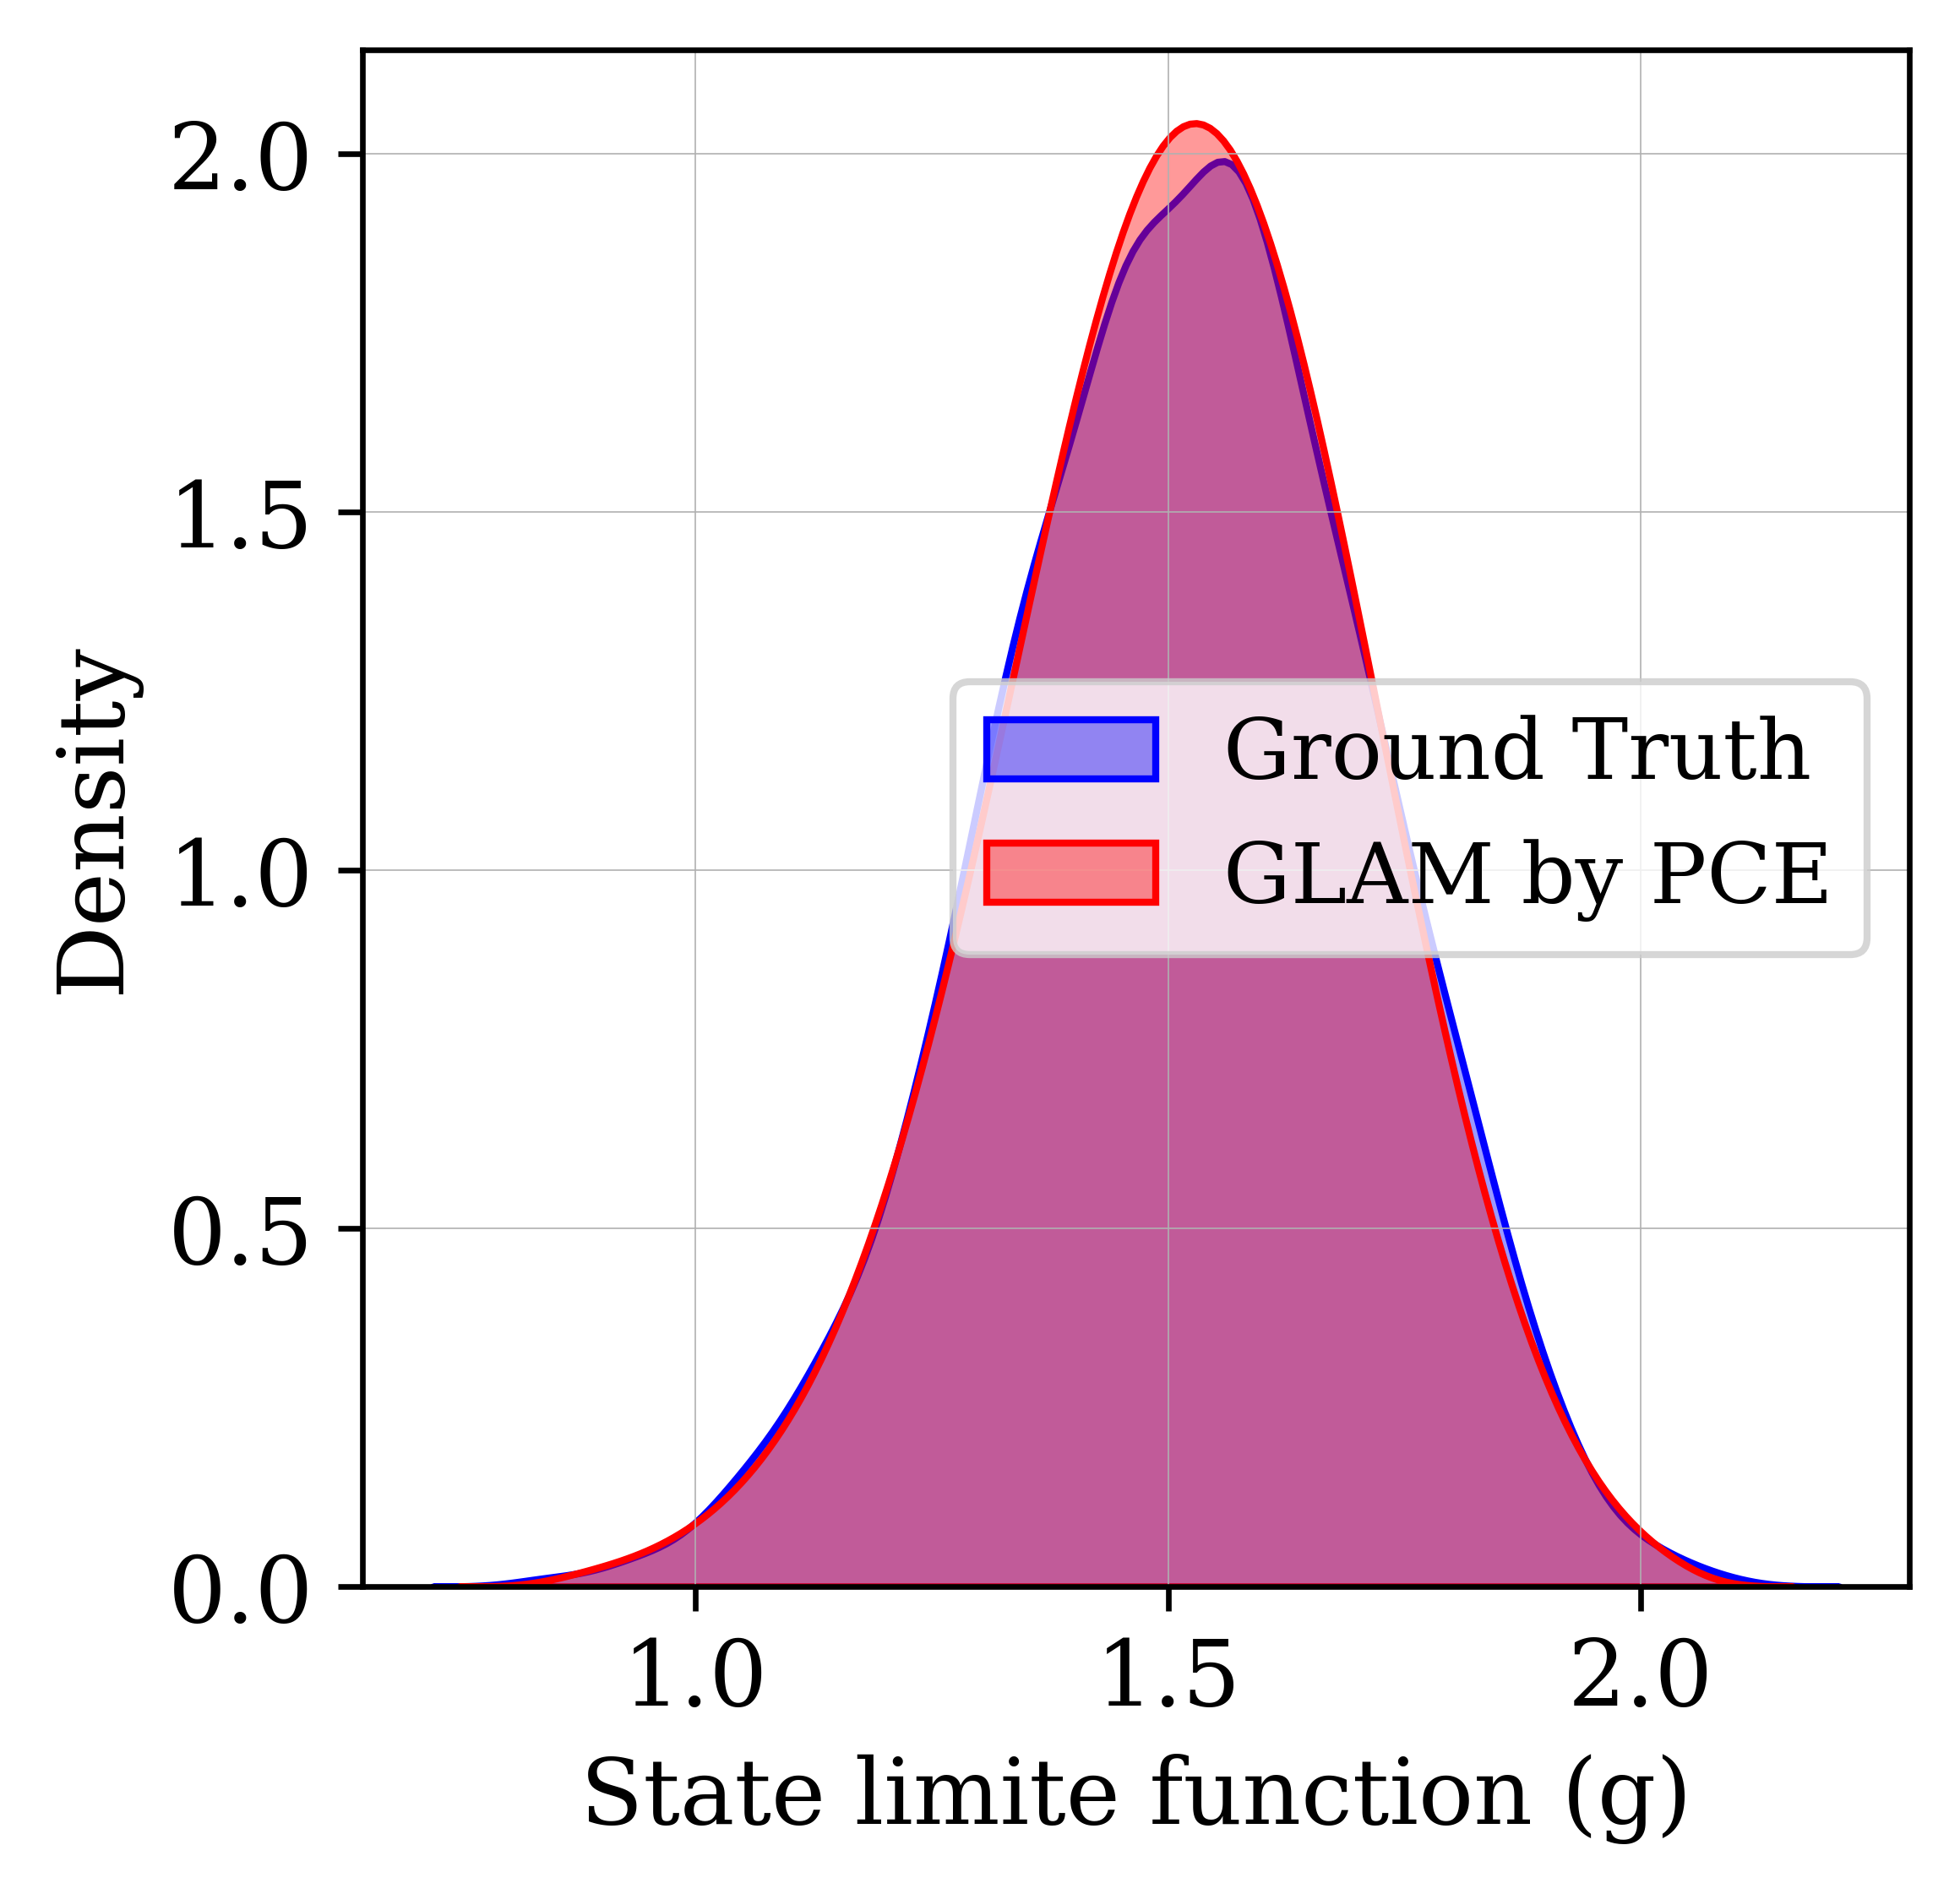
\includegraphics[width=\textwidth]{z_histogram_glam_versus_gt_t0_en.png}
        \caption{$t = 0$}
        \label{fig:kde_t0}
    \end{subfigure}
    \hfill
    \begin{subfigure}[b]{0.42\textwidth}
        \centering
        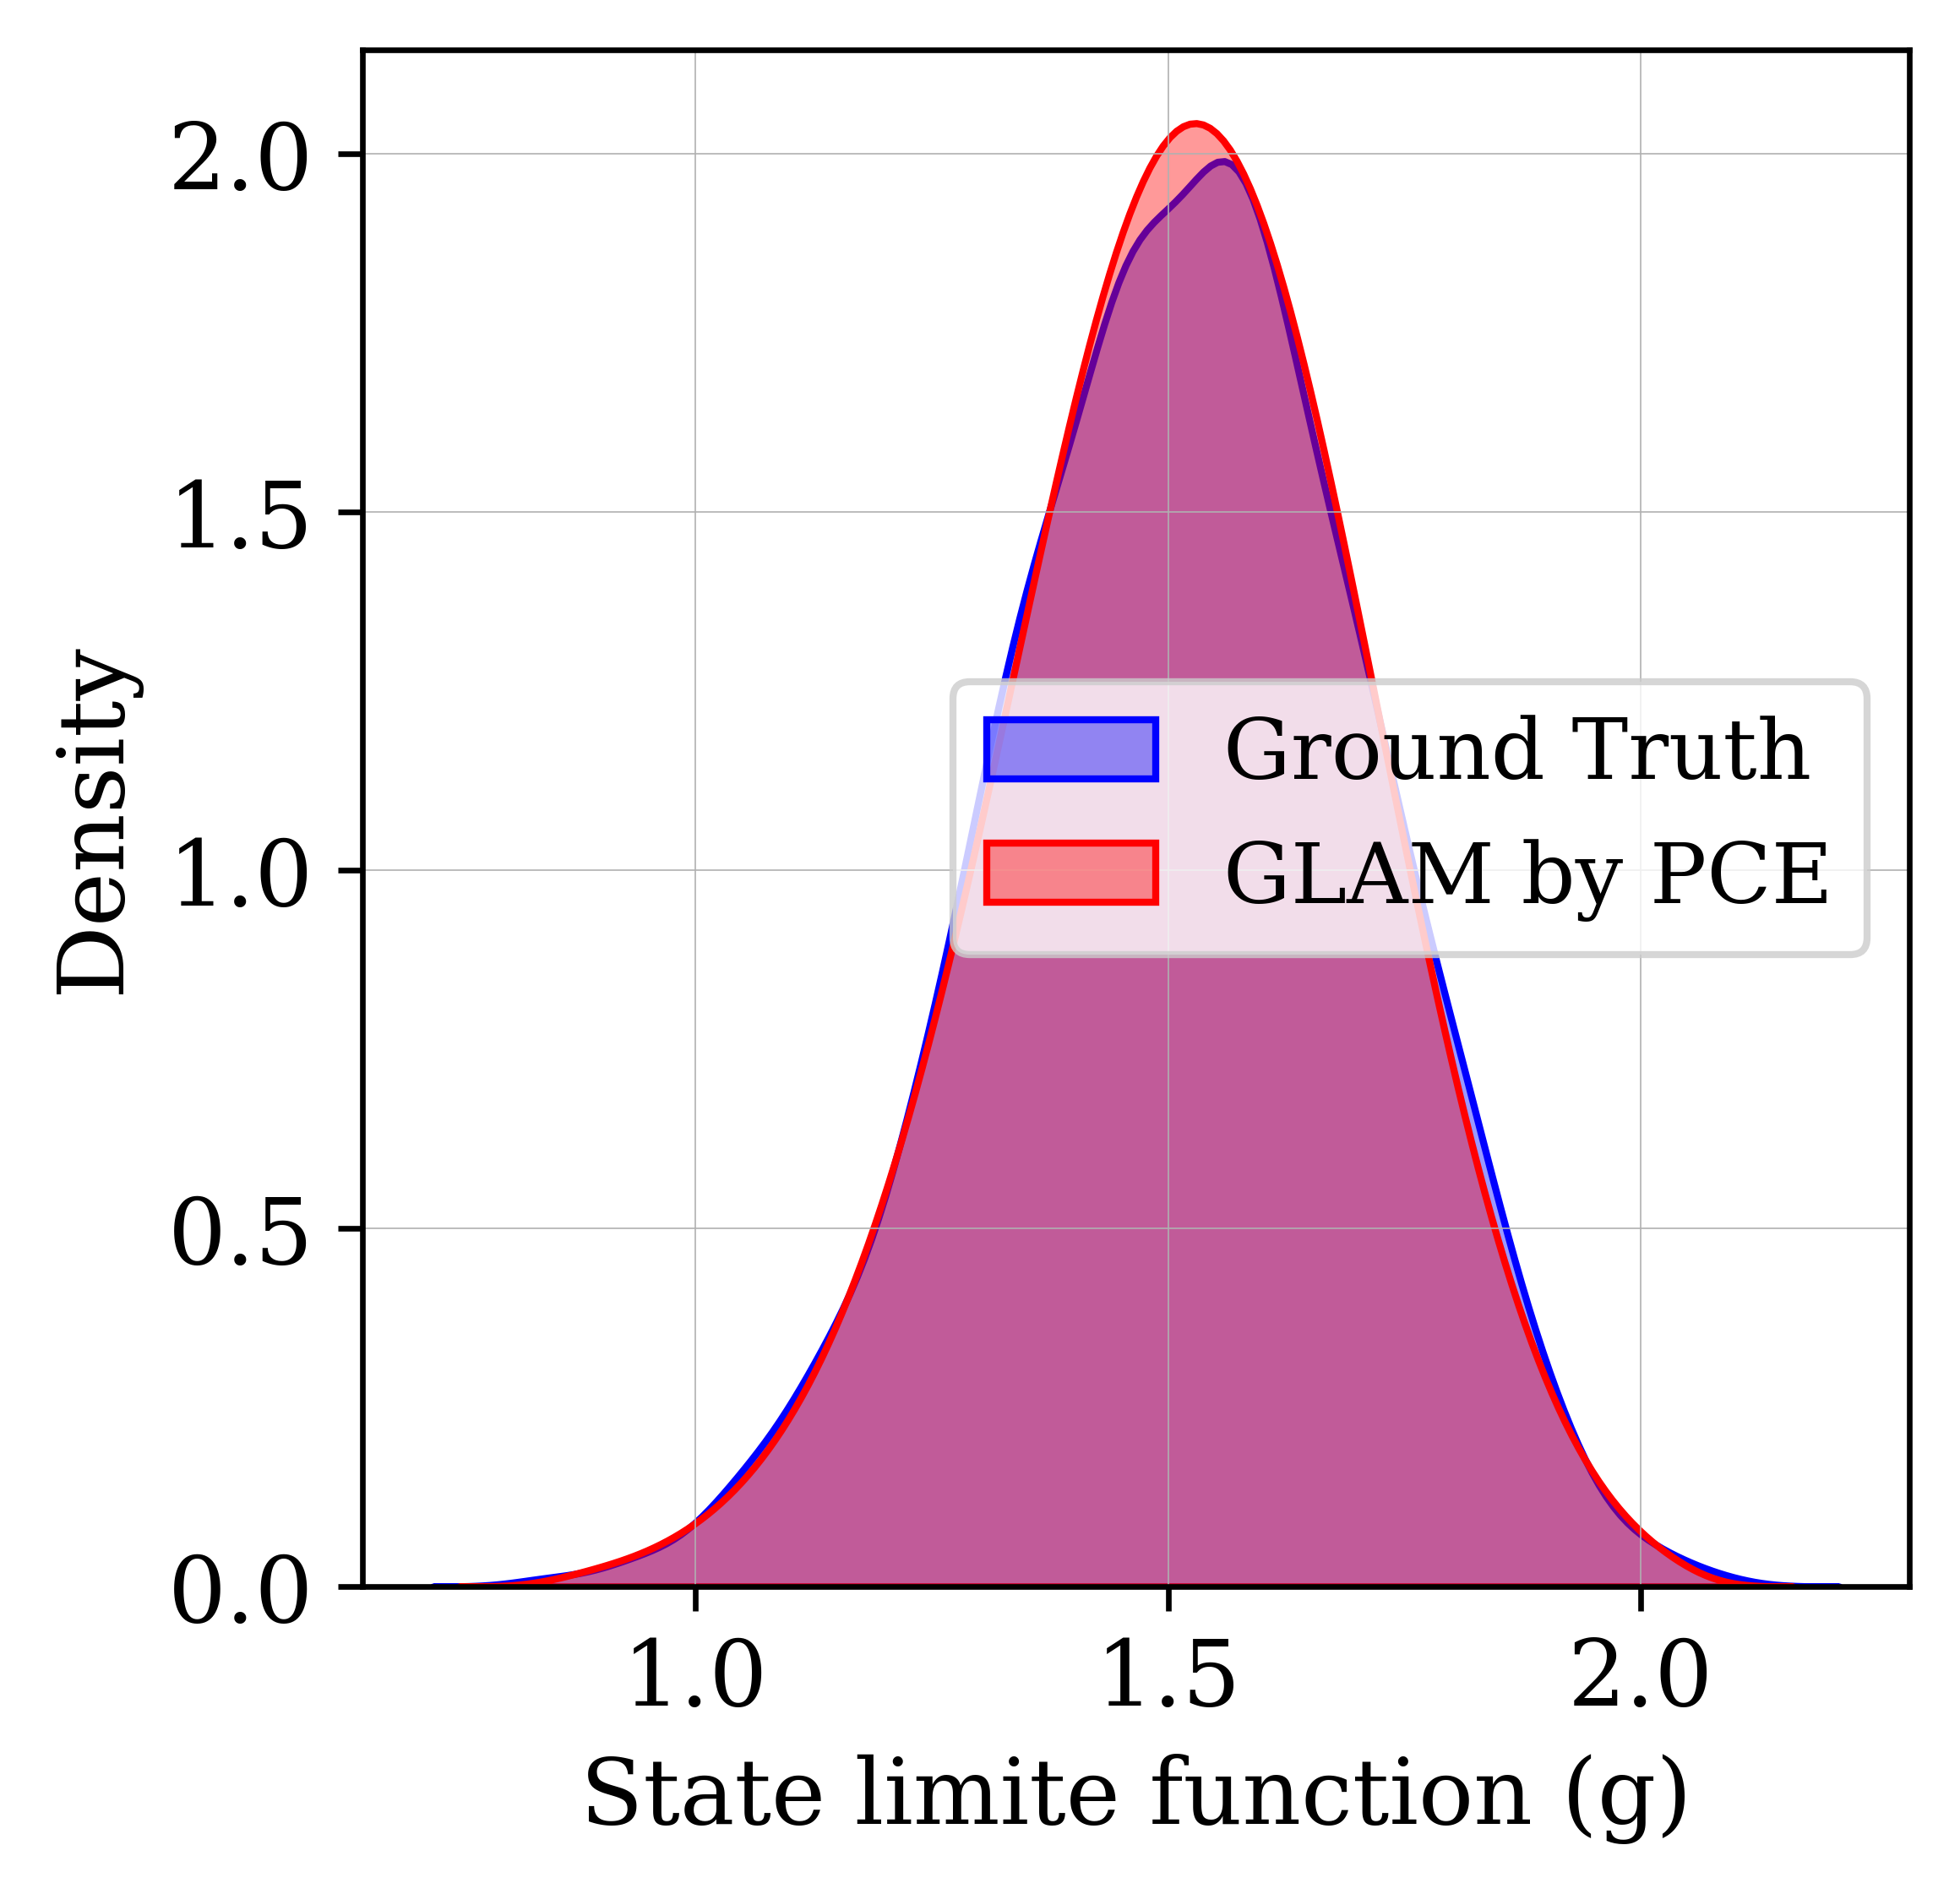
\includegraphics[width=\textwidth]{z_histogram_glam_versus_gt_t50_en.png}
        \caption{$t = 50$ anos}
        \label{fig:kde_t50}
    \end{subfigure}
    \vspace{0.2cm}
    \fonte{Autor (2025).}
\end{figure}

A similaridade estatística foi quantificada pelos testes de aderência e pela comparação de quantis descritos na \autoref{sec:metricas_emulador}, com resultados nas Tabelas \ref{tab:statistical_tests} e \ref{tab:quantile_comparison}. O teste de Kolmogorov--Smirnov não rejeita a hipótese nula ao nível de 5\% ($D = 0{,}0108$; valor-p $= 0{,}9325$), indicando excelente concordância global entre as funções de distribuição empíricas. O teste de Anderson--Darling, em contraste, rejeita a hipótese nula, comportamento atribuído à sua elevada sensibilidade às caudas em amostras grandes \cite{scholz1987}.

\begin{table}[H]
\centering
\caption{Testes de aderência entre a referência e o emulador.}
\label{tab:statistical_tests}
\begin{tabular}{lcccc}
\toprule
\textbf{Teste} & \textbf{Estatística} & \textbf{valor-p} & \textbf{Nível ($\alpha$)} & \textbf{Decisão} \\
\midrule
Kolmogorov--Smirnov & 0,0108      & 0,9325 & 0,05 & Não rejeita $H_0$ \\
Anderson--Darling   & $-0{,}6492$ & 0,0025 & 0,05 & Rejeita $H_0$ \\
\bottomrule
\end{tabular}
\vspace{0.2cm}
\fonte{Autor (2025).}
\end{table}

A análise de quantis localiza a origem dessa discrepância. Conforme a Tabela \ref{tab:quantile_comparison}, os erros relativos permanecem abaixo de 0,5\% até o percentil 99, subindo a cerca de 1,3\% apenas no quantil extremo de 99,9\% --- desvio confinado à cauda e usualmente considerado aceitável em análises de confiabilidade e quantificação de incertezas \cite{sudret2008}. Esse resultado é particularmente relevante para o presente trabalho, pois é justamente a cauda inferior da distribuição de $g$ que governa a probabilidade de falha.

\begin{table}[H]
\centering
\caption{Comparação de quantis entre a referência e o emulador.}
\label{tab:quantile_comparison}
\begin{tabular}{ccccc}
\toprule
\textbf{Quantil} & \textbf{Referência} & \textbf{Emulador} & \textbf{Dif. absoluta} & \textbf{Dif. relativa (\%)} \\
\midrule
0,001 & 0,8995 & 0,9037 & 0,0042 & 0,47 \\
0,010 & 1,0387 & 1,0393 & 0,0006 & 0,06 \\
0,500 & 1,5222 & 1,5198 & 0,0024 & 0,16 \\
0,990 & 1,9374 & 1,9356 & 0,0018 & 0,09 \\
0,999 & 2,0529 & 2,0263 & 0,0266 & 1,30 \\
\bottomrule
\end{tabular}
\vspace{0.2cm}
\fonte{Autor (2025).}
\end{table}

A divergência de Kullback--Leibler entre as distribuições de referência e emulada, prevista na \autoref{sec:metricas_emulador}, será incorporada a esta análise na etapa final da pesquisa, complementando as métricas de aderência já reportadas.

\subsection{Camada Temporal de Aprendizado de Máquina}

Partindo da análise em passos discretos via PCE, uma rede neural artificial foi adotada para viabilizar a predição contínua dos parâmetros $\lambda_1$ e $\lambda_2$ ao longo da vida útil, conforme a formulação da \autoref{RNA}. Para o treinamento, uma base sintética de 11.000 amostras foi gerada com os metamodelos PCE previamente validados, amostrando-se o espaço de entrada segundo as distribuições da Tabela \ref{tab:random_variables_parameters} e valores de tempo uniformemente distribuídos no horizonte de análise. A rede mapeia o vetor de entrada $\mathbf{z} = \{R, S, t\}$ no vetor de saída $\{\lambda_1, \lambda_2\}$, com partição aleatória em subconjuntos de treinamento e teste na mesma proporção de 70/30 adotada na \autoref{sec:res_ml}.

A Figura \ref{fig:ann_temporal} ilustra a evolução temporal de $\lambda_1$ e $\lambda_2$ ao longo dos 100 anos de vida útil, prevista pela rede treinada para o cenário representativo ($r = 5{,}09$, $s = 1{,}80$). A rede atua como interpolador contínuo, reconstruindo suavemente a trajetória de degradação entre os passos discretos originalmente avaliados pela PCE, sem ruído numérico ou descontinuidades. Quantitativamente, o modelo atingiu $R^2 = 0{,}9976$ para $\lambda_1$ e $R^2 = 0{,}9844$ para $\lambda_2$ no conjunto de teste, validando a rede neural como interpolador robusto para a avaliação contínua da confiabilidade em qualquer instante do horizonte.

\begin{figure}[H]
    \centering
    \caption{Evolução temporal dos parâmetros $\lambda_1$ e $\lambda_2$ ao longo da vida útil.}
    \label{fig:ann_temporal}
    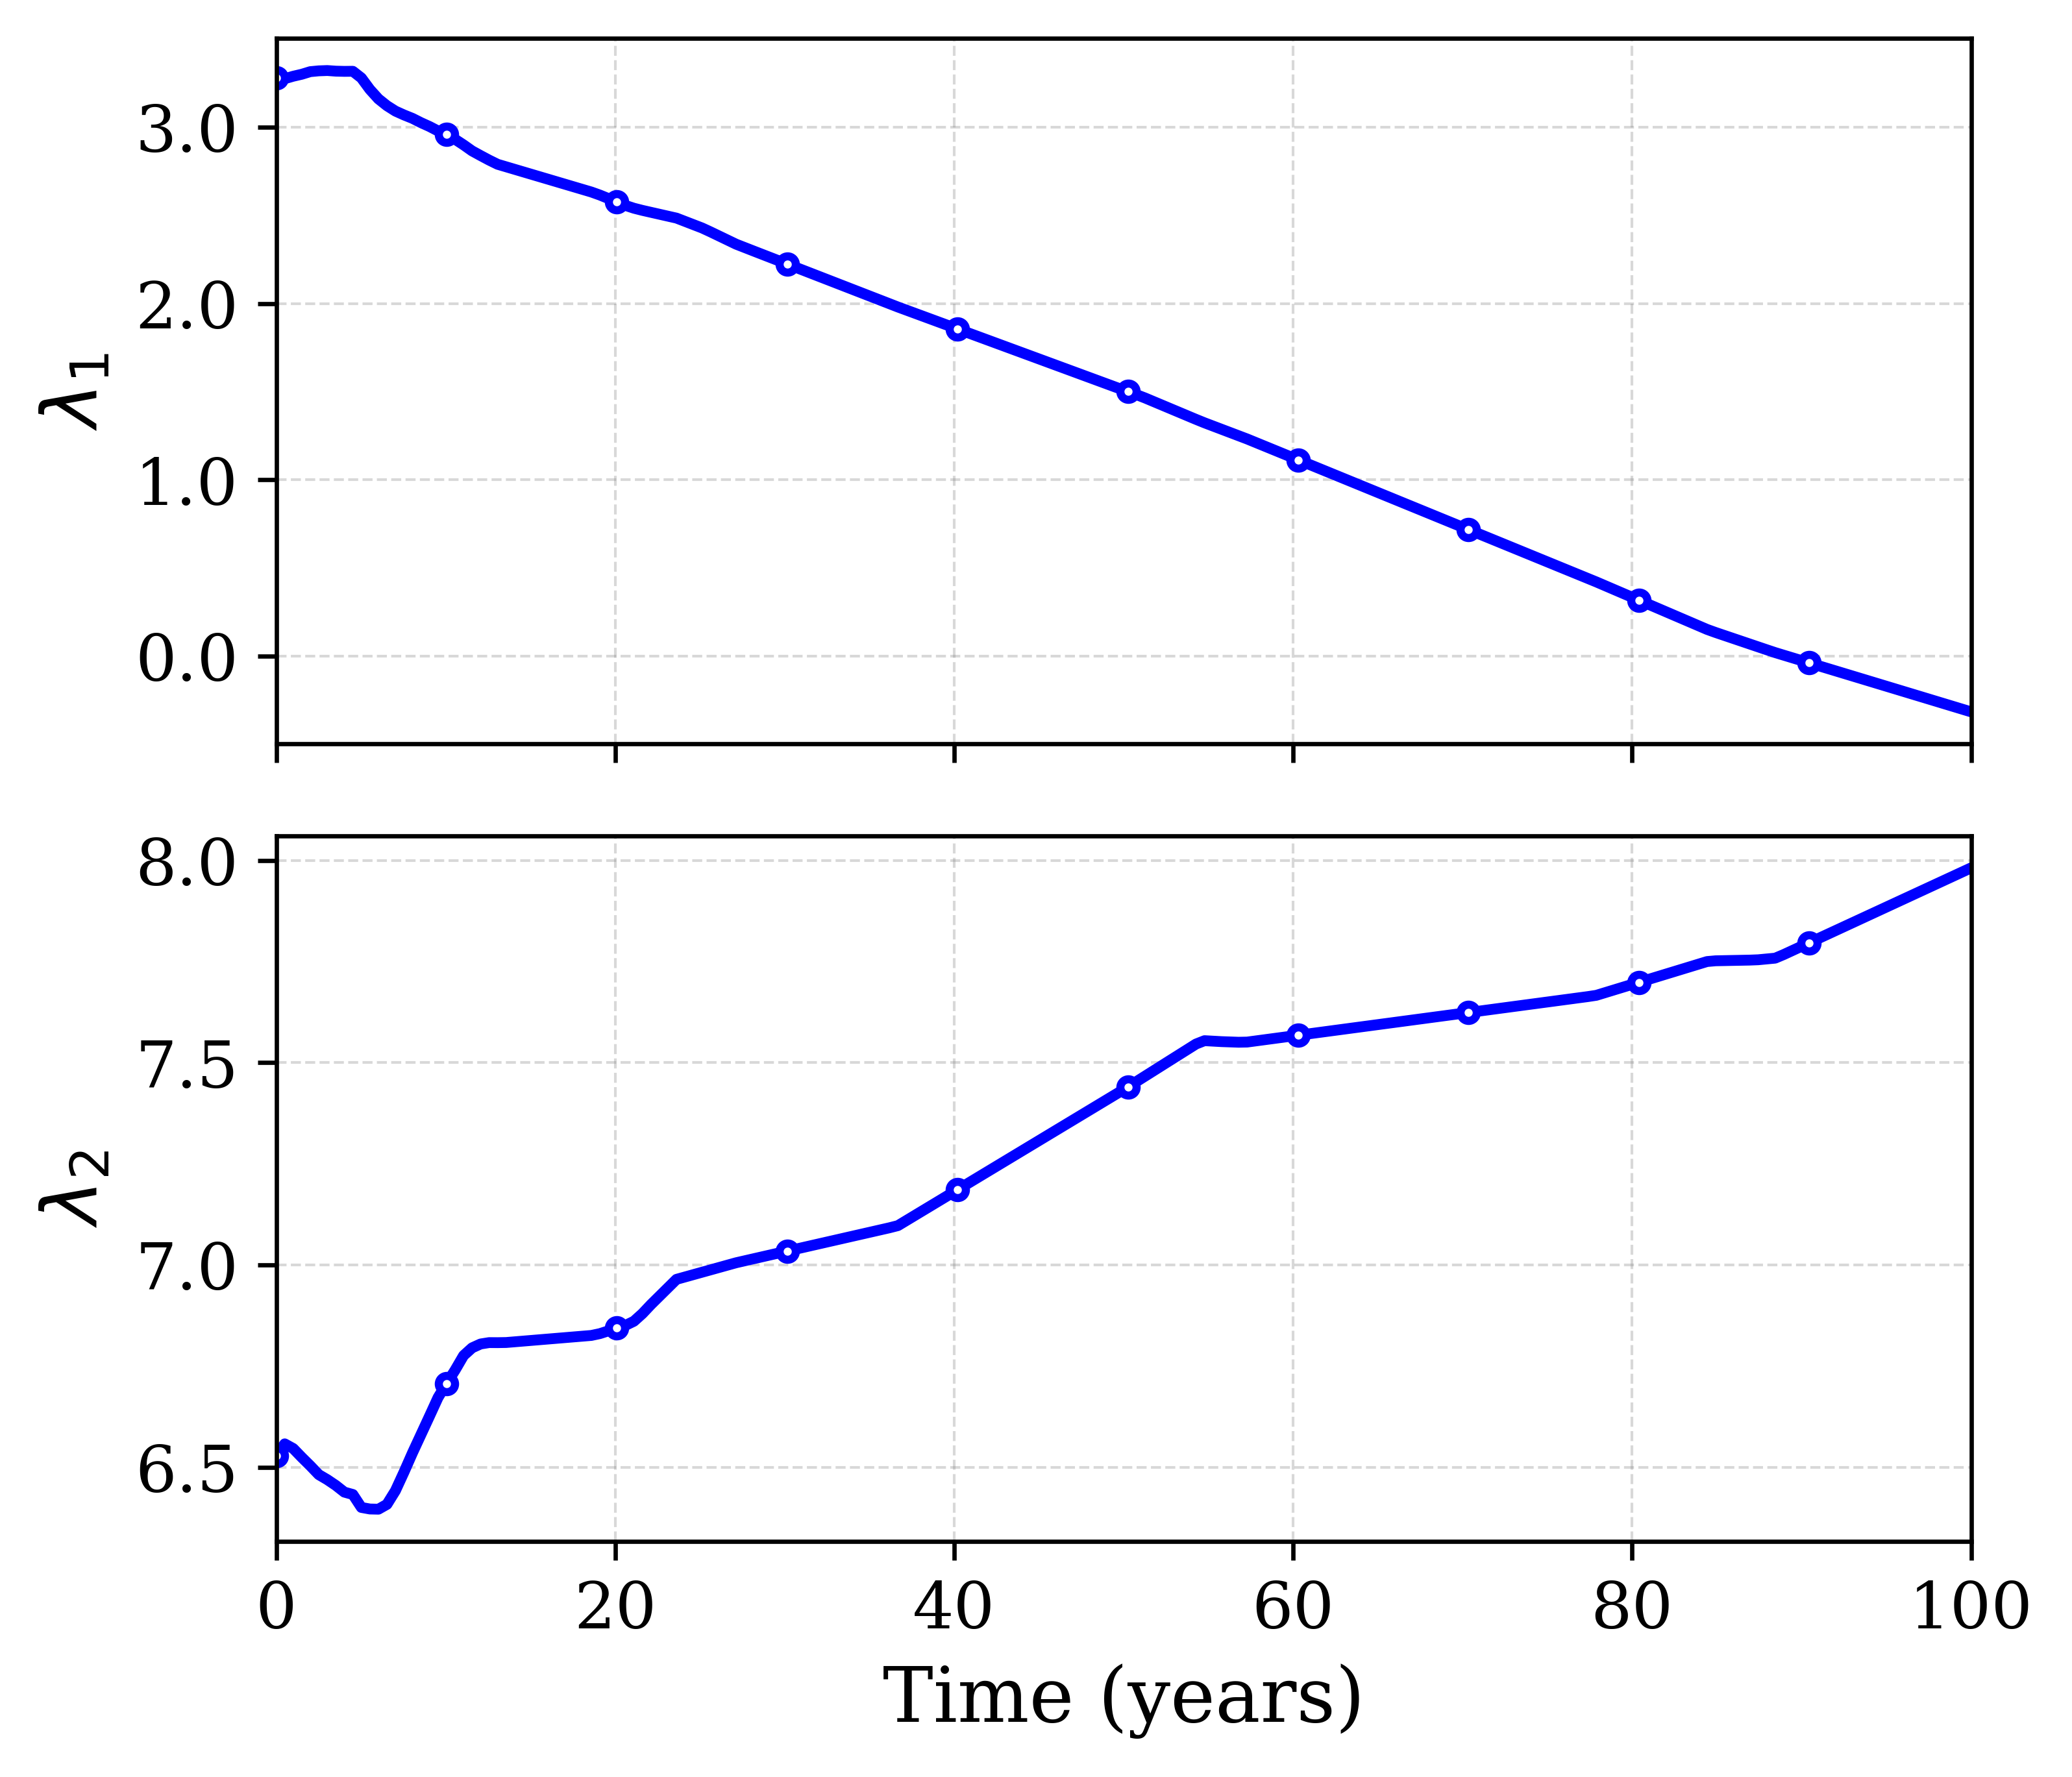
\includegraphics[width=0.75\linewidth]{z_temporal_evolution_ann_with_points_en.png}
    \vspace{0.2cm}
    \fonte{Autor (2025).}
\end{figure}

Cabe registrar que o teste mais exigente da capacidade de emulação temporal --- treinar a rede \textit{omitindo} deliberadamente um ou dois passos de tempo e comparar a densidade prevista nesses anos com a simulação direta de Monte Carlo --- ainda não foi executado. Esse experimento, previsto no cronograma revisado, é o que sustenta de forma conclusiva a alegação de emulação contínua no tempo e será conduzido tanto para o problema de referência quanto para o problema da viga.

\subsection{Vida Útil Remanescente e Custo Computacional}

Aplicando a metodologia da \autoref{sec:emulador_rul}, a Figura \ref{fig:rul_results} apresenta os produtos probabilísticos do arcabouço: a distribuição da função de estado limite no instante de inspeção de 35 anos, adotado como exemplo representativo; a densidade de probabilidade do tempo até a falha, obtida pela identificação do instante em que a trajetória de $g$ se anula, conforme a Equação \eqref{eq:ttf}; e a distribuição resultante da vida útil remanescente, Equação \eqref{eq:rul}, que consolida as incertezas propagadas e constitui o resultado central para a manutenção preditiva.

\begin{figure}[H]
    \centering
    \caption{Resultados probabilísticos do arcabouço baseado em emulador para a estimativa da VUR.}
    \label{fig:rul_results}
    \begin{subfigure}[b]{0.32\textwidth}
        \centering
        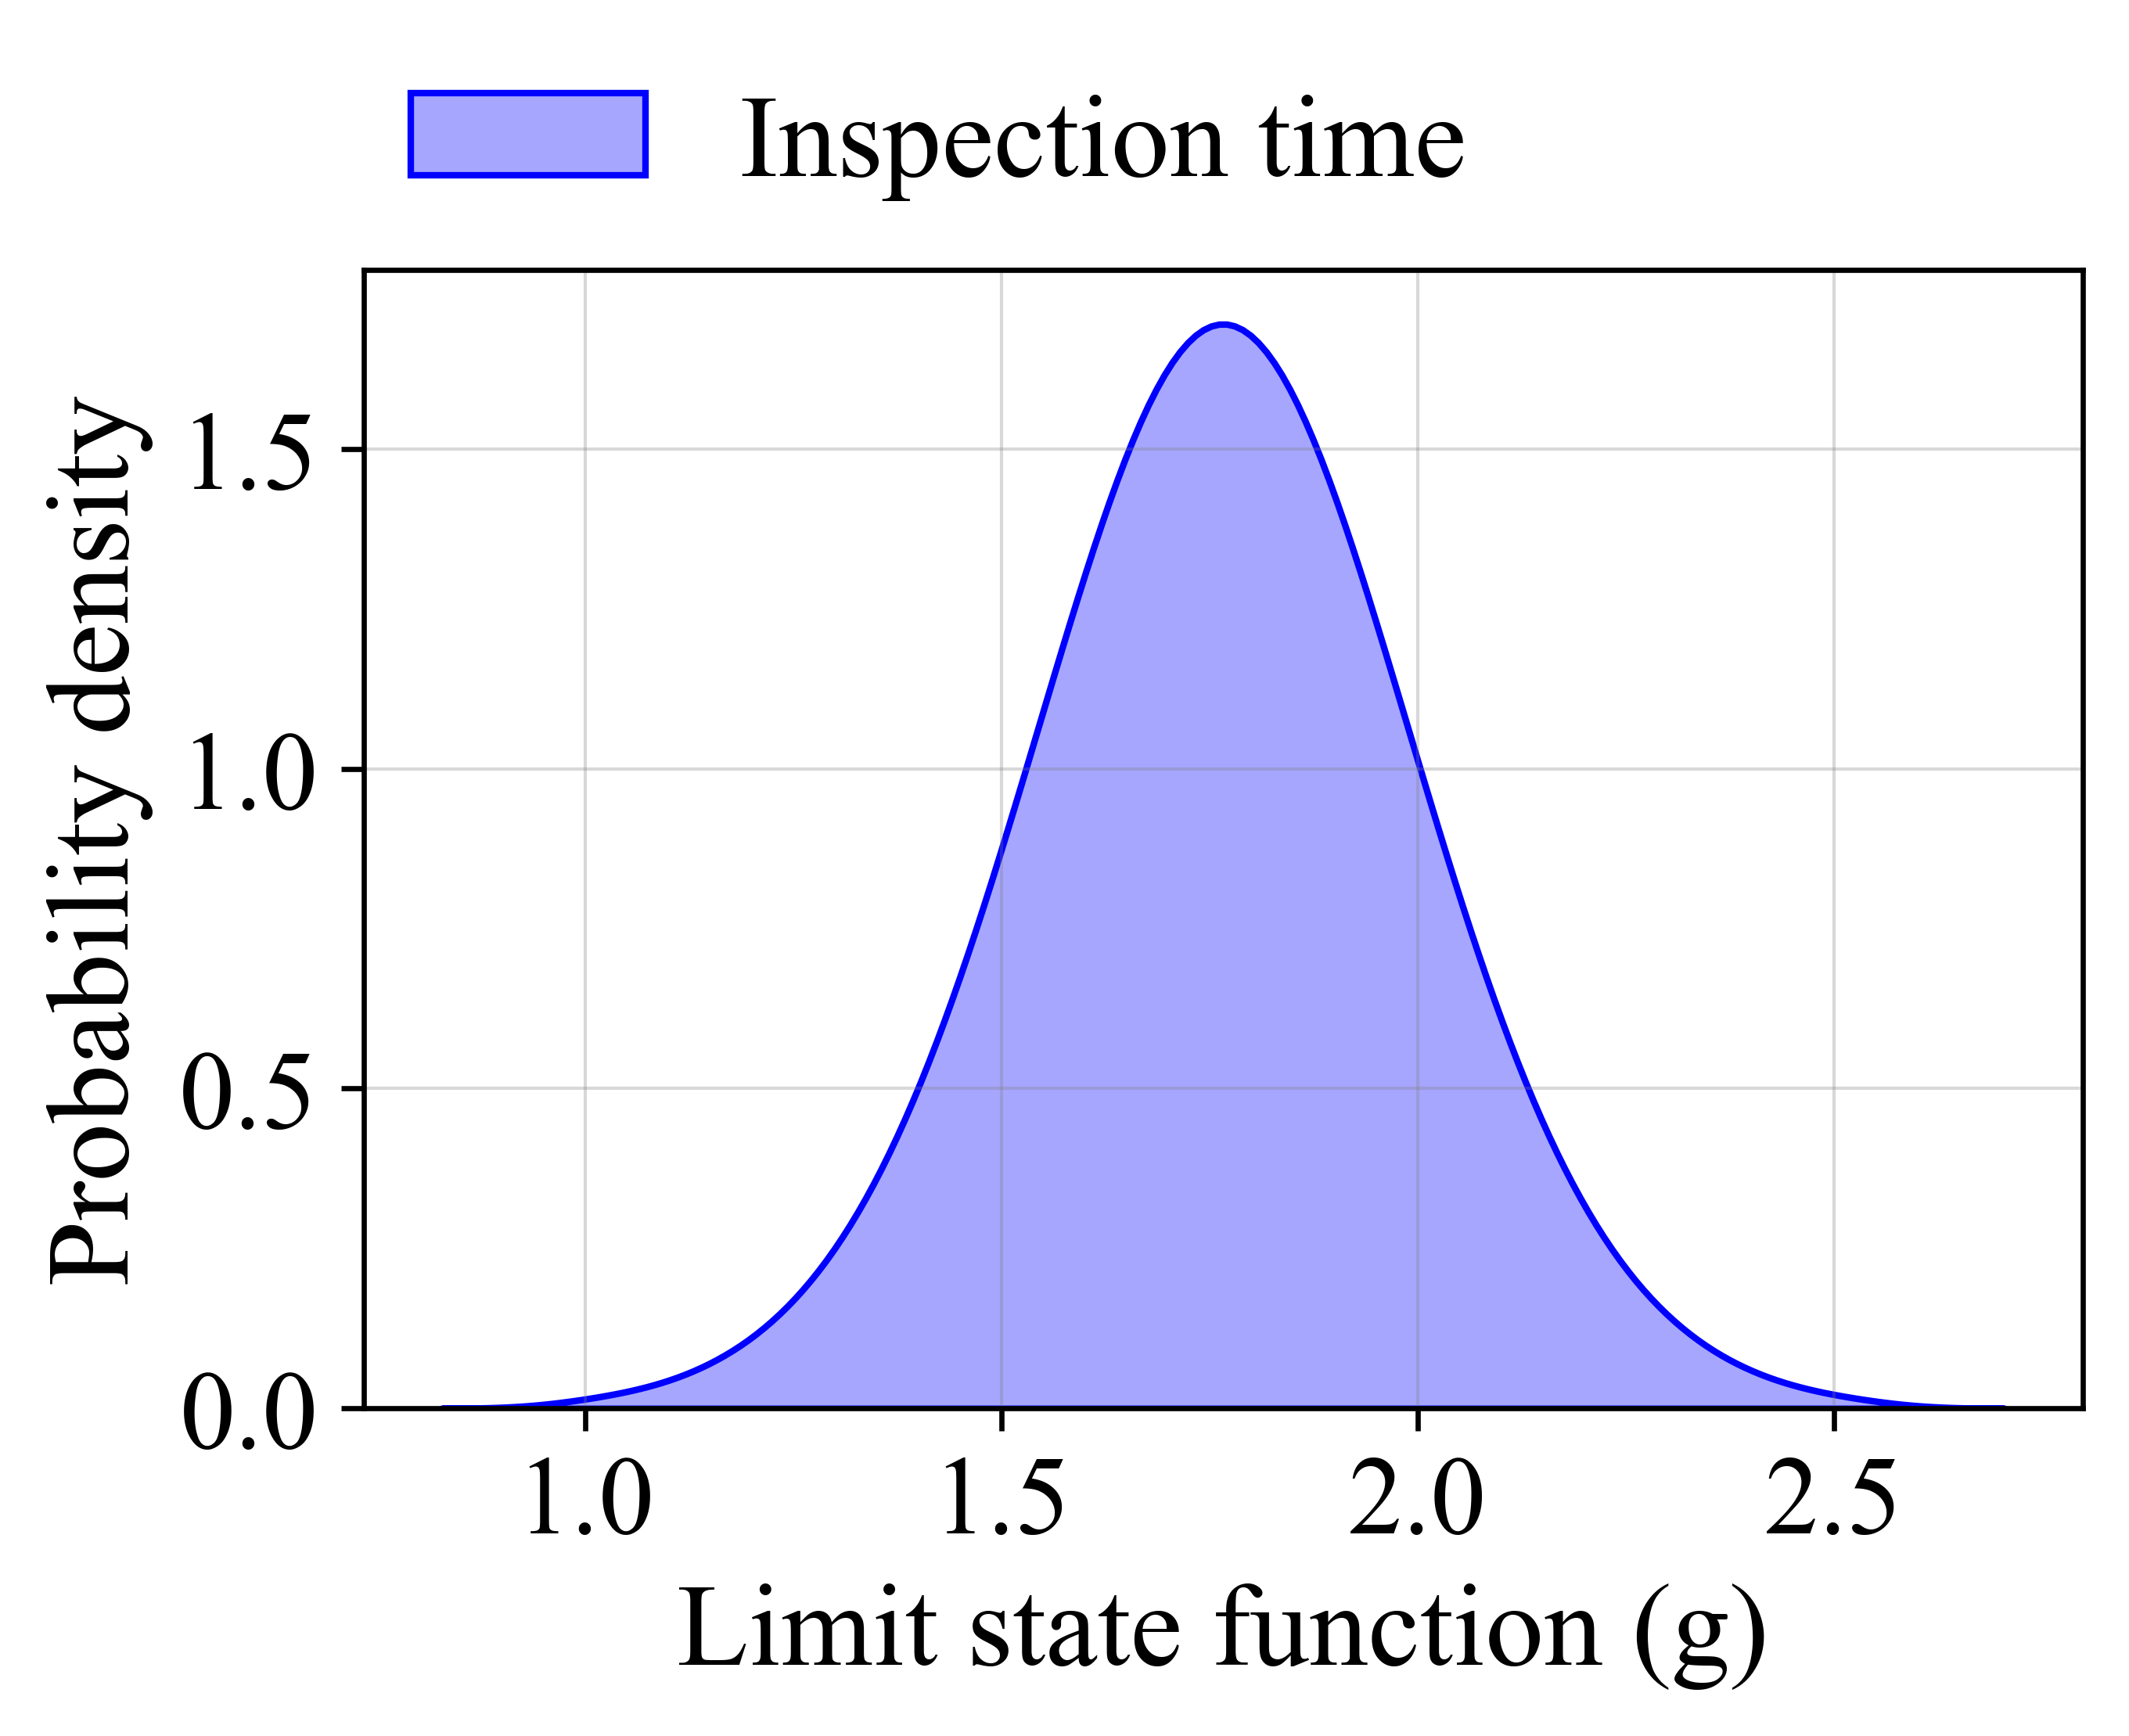
\includegraphics[height=4.0cm,keepaspectratio]{z_kde_inspection_time.png}
        \caption{$g$ no instante de inspeção.}
        \label{fig:kde_inspection_time}
    \end{subfigure}
    \hfill
    \begin{subfigure}[b]{0.32\textwidth}
        \centering
        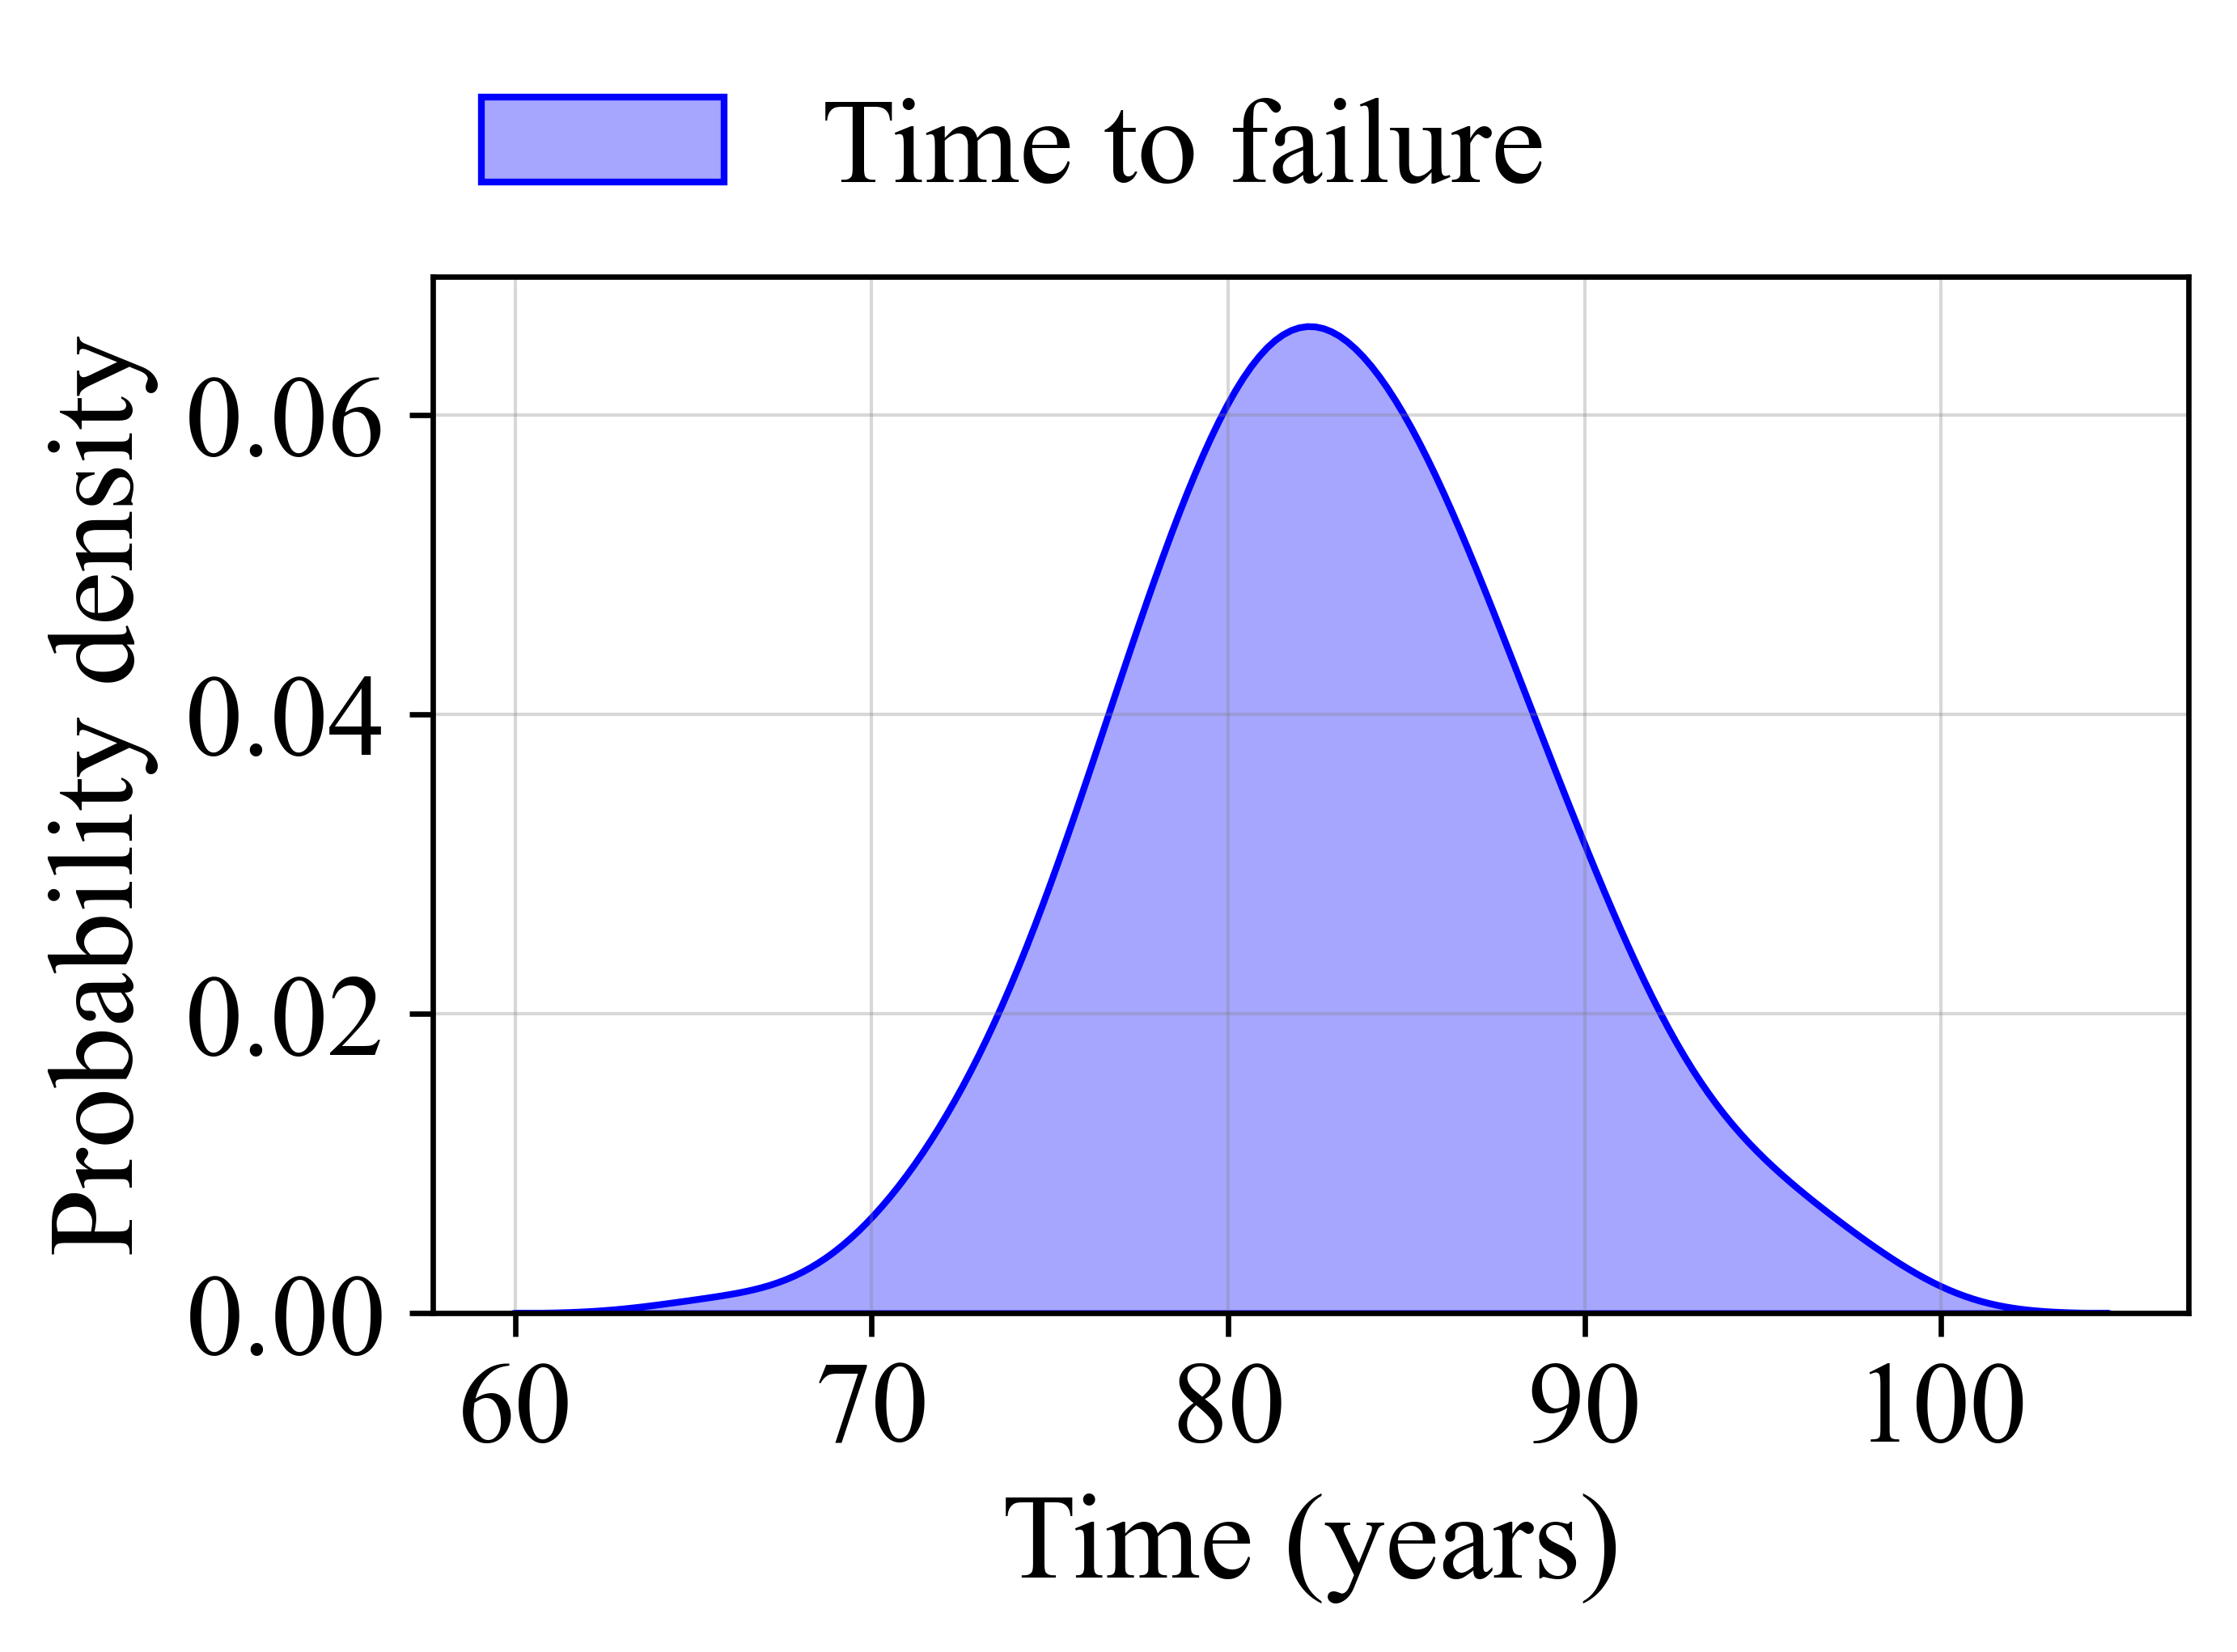
\includegraphics[height=4.0cm,keepaspectratio]{z_kde_time_to_failure.png}
        \caption{Tempo até a falha.}
        \label{fig:kde_time_to_failure}
    \end{subfigure}
    \hfill
    \begin{subfigure}[b]{0.32\textwidth}
        \centering
        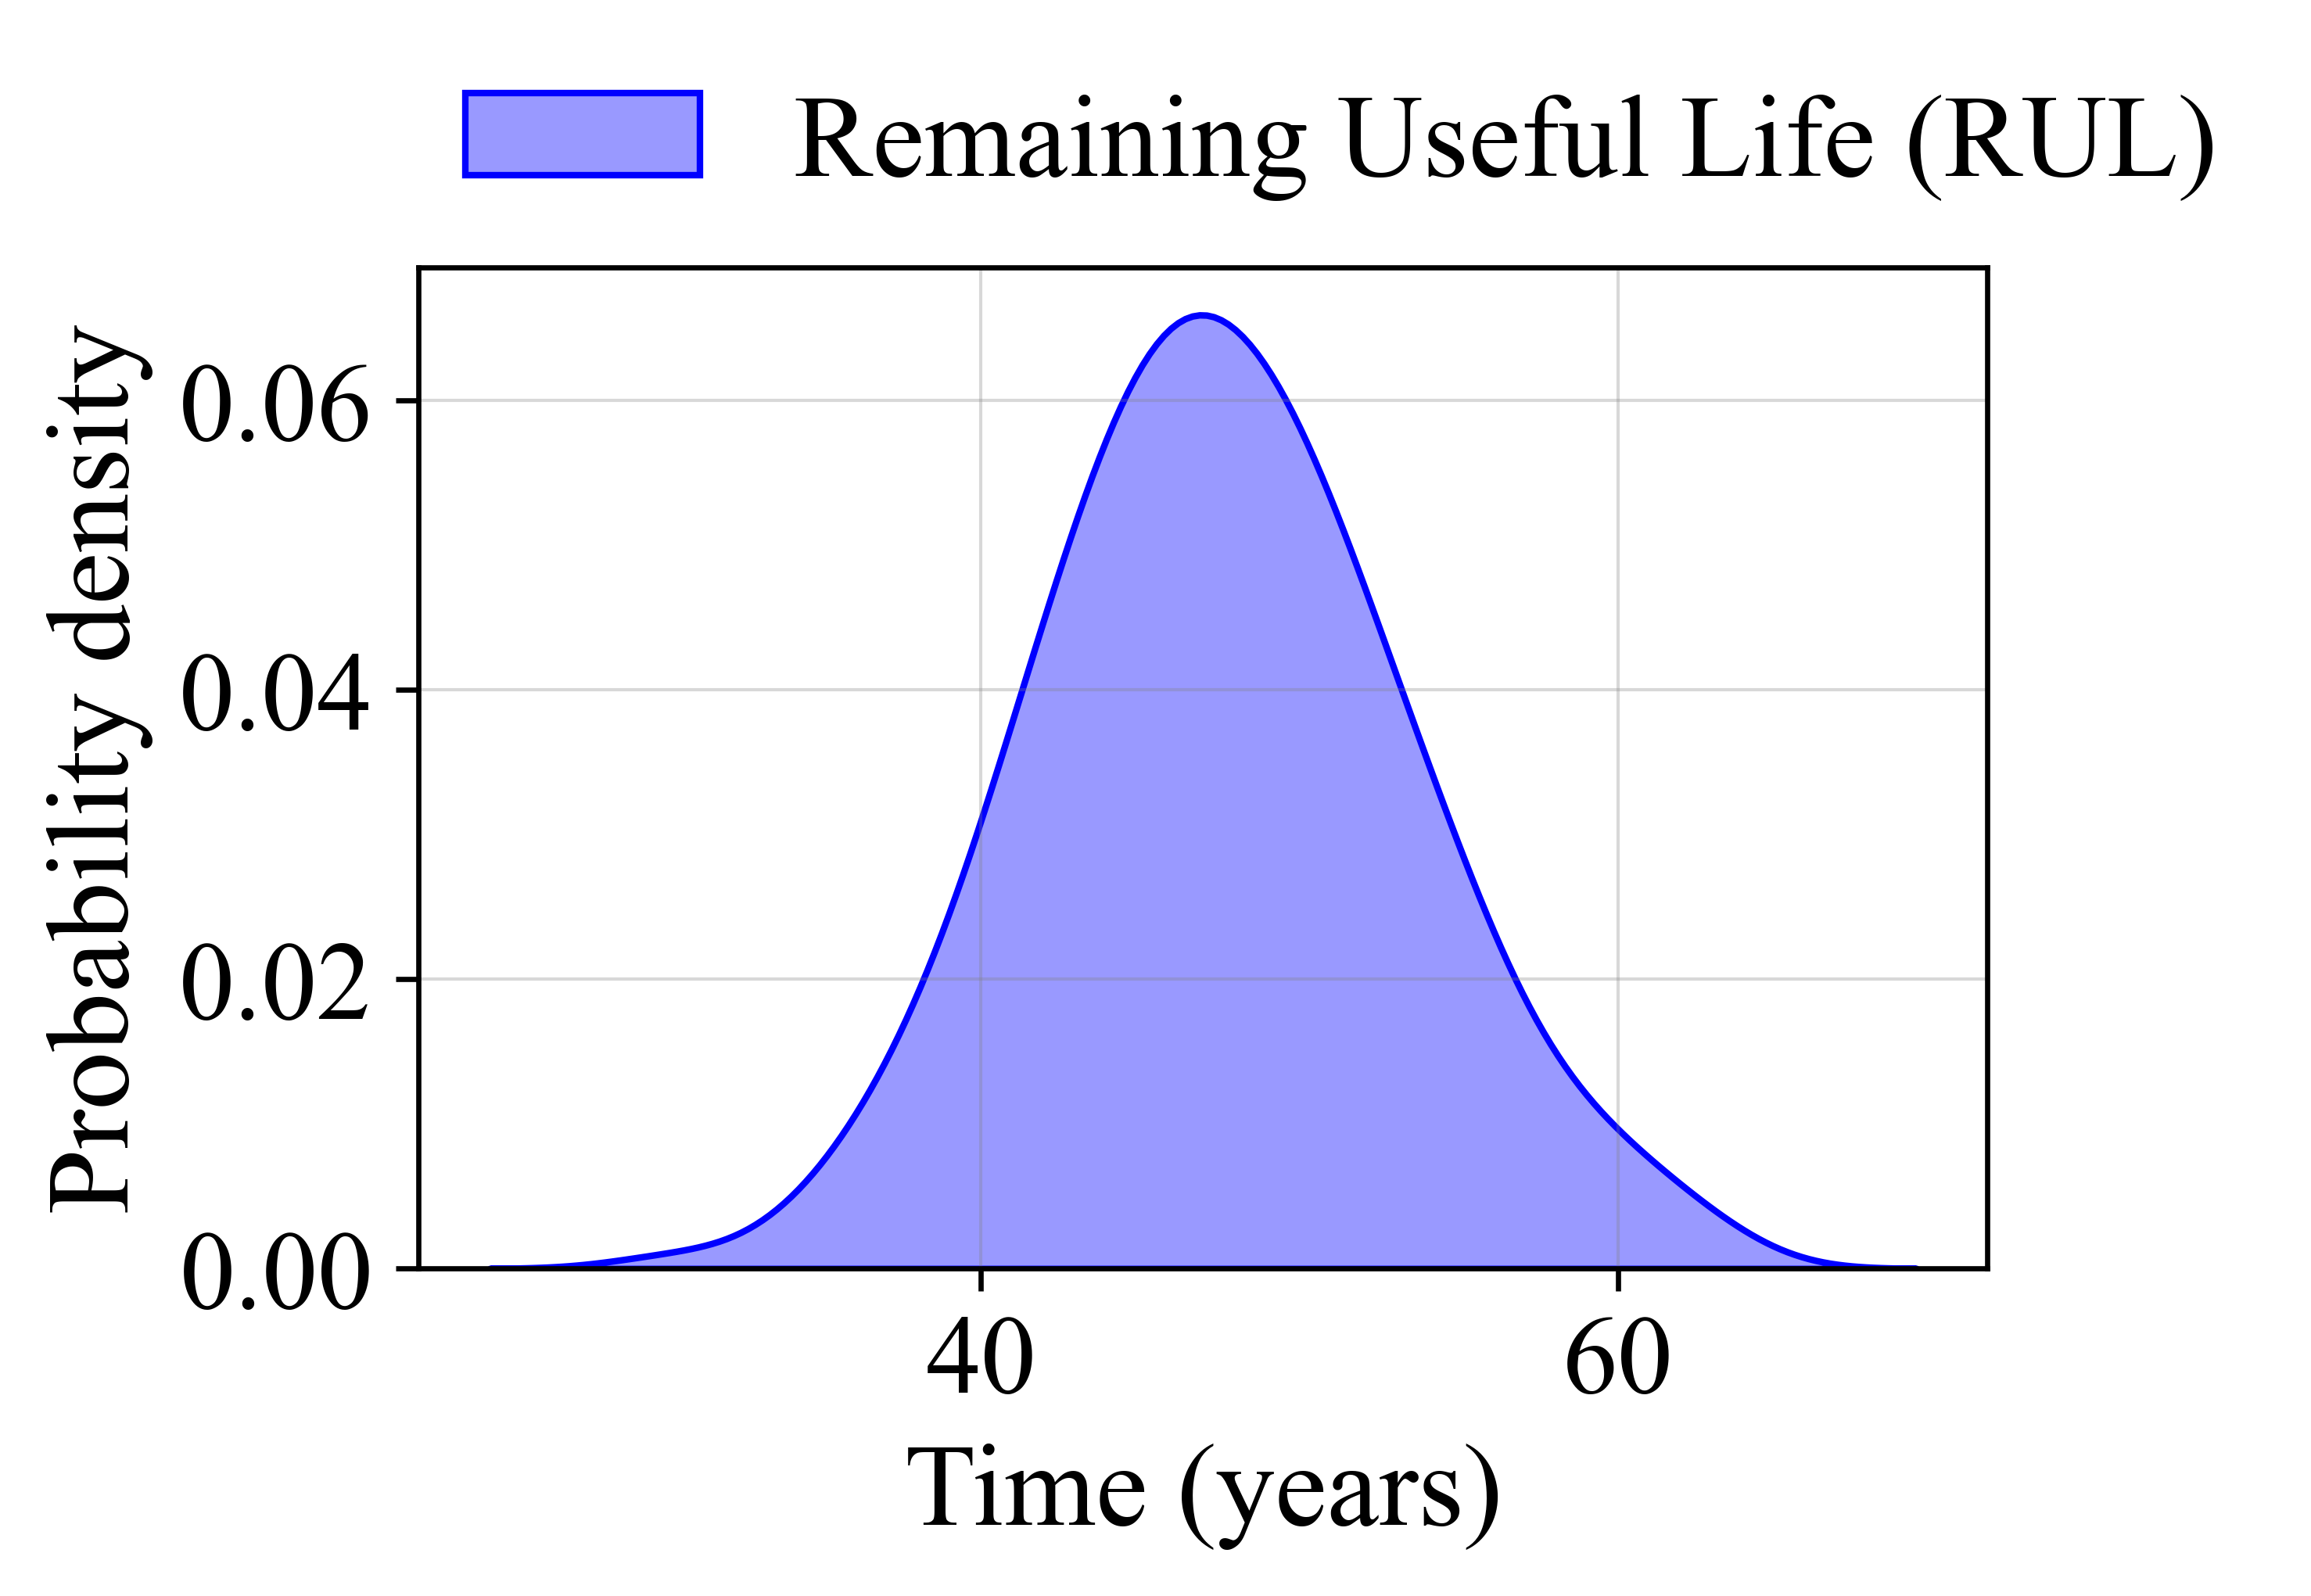
\includegraphics[height=4.0cm,keepaspectratio]{z_kde_rul.png}
        \caption{Vida útil remanescente.}
        \label{fig:kde_rul}
    \end{subfigure}
    \vspace{0.2cm}
    \fonte{Autor (2025).}
\end{figure}

Nota-se a correspondência conceitual direta entre esses três painéis e os histogramas apresentados na \autoref{sec:res_vur}: as mesmas três estatísticas de interesse --- tempo total de vida útil, valor da função de estado limite em um instante genérico e vida útil condicional --- são agora obtidas por avaliação analítica da função quantílica emulada, e não por contagem sobre amostras de Monte Carlo.

As métricas de risco derivadas da distribuição de VUR para $\alpha = 5\%$ são apresentadas na Tabela \ref{tab:var_cvar_rul}. A diferença relativamente pequena entre VaR e CVaR sugere severidade de cauda limitada, indicando que, mesmo em condições desfavoráveis, a vida remanescente prevista não exibe degradação abrupta.

\begin{table}[H]
\centering
\caption{Métricas de risco derivadas da distribuição de VUR para $\alpha = 5\%$.}
\label{tab:var_cvar_rul}
\begin{tabular}{lc}
\toprule
\textbf{Métrica} & \textbf{Valor (anos)} \\
\midrule
VaR$_{5\%}$  & 38,38 \\
CVaR$_{5\%}$ & 36,42 \\
\bottomrule
\end{tabular}
\vspace{0.2cm}
\fonte{Autor (2025).}
\end{table}

Além da acurácia das predições probabilísticas, o arcabouço oferece ganho substancial de eficiência computacional. A Tabela \ref{tab:computational_time} compara o tempo de processamento exigido pela abordagem convencional de simulação direta e pelo emulador: enquanto o procedimento convencional demandou aproximadamente 48,75~s, o emulador reduziu o custo a apenas 0,66~s, correspondendo a uma aceleração de quase duas ordens de grandeza. Esse resultado evidencia a adequação da abordagem a análises de confiabilidade e de vida útil remanescente em tempo quase real ou em larga escala, e é precisamente o que viabiliza a varredura de cenários de inspeção e manutenção pretendida na etapa final da pesquisa.

\begin{table}[H]
\centering
\caption{Comparação do tempo computacional entre a abordagem convencional e a baseada em emulador.}
\label{tab:computational_time}
\begin{tabular}{lc}
\toprule
\textbf{Método} & \textbf{Tempo computacional (s)} \\
\midrule
Abordagem convencional (Monte Carlo direto) & 48,75 \\
Abordagem com emulador                      & 0,66 \\
\bottomrule
\end{tabular}
\vspace{0.2cm}
\fonte{Autor (2025).}
\end{table}

\section{Aplicação do Emulador à Viga sob Carbonatação: Estado de Desenvolvimento} \label{sec:res_emulador_viga}

Verificado o arcabouço metodológico no problema de referência, a etapa seguinte consiste em aplicar o emulador ao problema-alvo desta dissertação: a previsão da vida útil remanescente de uma viga de concreto armado sujeita à corrosão induzida por carbonatação, com a função de estado limite da Equação \eqref{eq:estado_limite} e os modelos físicos apresentados no \autoref{cap:referencial}. Esta seção documenta o estado atual dessa aplicação e o que resta a ser executado.

\subsection{Etapas Concluídas}

Encontram-se concluídas as seguintes etapas, descritas nos capítulos anteriores:

\begin{alineas}
    \item a implementação do simulador estocástico completo, integrando o modelo de avanço da frente de carbonatação, a perda de seção e de aderência das armaduras e a verificação do estado limite último de flexão;
    \item a caracterização probabilística das variáveis básicas do problema, apresentada na Tabela \ref{tab:estatisticas_vars};
    \item a construção do banco de dados sintético por simulação de Monte Carlo com Hipercubo Latino e a extração das estatísticas de vida útil, conforme a \autoref{sec:res_vur};
    \item a implementação e a verificação da biblioteca PyGLAM para o ajuste da GLD pelo Método dos Momentos, incluindo os ensaios de aderência a distribuições-alvo conhecidas apresentados na Figura \ref{fig:pyglam_fits};
    \item a verificação do emulador PCE--GLD com camada temporal em problema de referência, conforme a \autoref{sec:res_emulador}.
\end{alineas}

\subsection{Etapas em Execução}

A transposição do emulador do problema de referência para o problema da viga apresenta duas diferenças relevantes que motivam tratamento cuidadoso. A primeira é a dimensionalidade: enquanto o problema de referência possui duas variáveis de entrada controladas, o problema da viga envolve o conjunto de variáveis geométricas, mecânicas e ambientais da Tabela \ref{tab:estatisticas_vars}, o que amplia o número de coeficientes da PCE e exige plano de experimentos mais extenso. A segunda é a natureza descontínua da função de estado limite adotada, Equação \eqref{eq:estado_limite}, cuja mudança de regime no instante de despassivação introduz um ponto de não suavidade na trajetória temporal de $g$ --- o que demanda verificação específica da capacidade da camada temporal de reproduzir essa transição.

As atividades em execução para superar esses pontos são as seguintes:

\begin{alineas}
    \item definição do plano de experimentos final, com determinação do número $M$ de pontos amostrais, do número $N$ de réplicas por ponto e dos $N_t$ passos de tempo, mediante estudo de convergência;
    \item repetição da análise exploratória de sensibilidade dos parâmetros da GLD, a fim de confirmar ou refutar, no problema da viga, a baixa variabilidade de $\lambda_3$ e $\lambda_4$ observada no problema de referência;
    \item comparação sistemática de regressores para a camada temporal --- rede neural, floresta aleatória e regressão por vetores de suporte --- com otimização de hiperparâmetros pelo mesmo procedimento adotado na \autoref{sec:res_ml};
    \item validação do emulador em instantes deliberadamente excluídos do treinamento, com comparação contra Monte Carlo direto e ênfase na cauda inferior da distribuição, região que governa a probabilidade de falha;
    \item obtenção das curvas de $p_f(t)$ e $\beta(t)$ emuladas, da distribuição do tempo até a falha e da distribuição de VUR para diferentes instantes de inspeção;
    \item análise de sensibilidade global por índices de Sobol, obtidos analiticamente dos coeficientes da PCE \cite{sudret2008}, para quantificar a contribuição de cada variável ao longo das fases de iniciação e de propagação da corrosão;
    \item avaliação de cenários de intervenção de manutenção e determinação do instante normativo de intervenção pela Equação \eqref{eq:t_man_otimo}.
\end{alineas}

A Tabela \ref{tab:estado_desenvolvimento} sintetiza o estágio de cada produto previsto para esta frente da pesquisa.

\begin{table}[H]
\centering
\footnotesize
\caption{Estágio de desenvolvimento dos produtos da frente de emulação estocástica.}
\label{tab:estado_desenvolvimento}
\begin{tabularx}{\textwidth}{X l}
\toprule
\textbf{Produto} & \textbf{Situação} \\
\midrule
Biblioteca PyGLAM (ajuste da GLD pelo Método dos Momentos)      & Concluído \\
Verificação do emulador PCE--GLD em problema de referência       & Concluído \\
Camada temporal por rede neural (problema de referência)          & Concluído \\
Distribuição de VUR e métricas de risco (problema de referência)  & Concluído \\
Teste de generalização em instantes omitidos do treinamento       & Em execução \\
Plano de experimentos do problema da viga                         & Em execução \\
Comparação de regressores para a camada temporal                  & Em execução \\
Curvas de $p_f(t)$ e $\beta(t)$ emuladas para a viga              & Previsto \\
Distribuição de VUR da viga sob carbonatação                      & Previsto \\
Análise de sensibilidade por índices de Sobol                     & Previsto \\
Cenários de intervenção de manutenção                             & Previsto \\
\bottomrule
\end{tabularx}
\vspace{0.2cm}
\fonte{Autor (2025).}
\end{table}

\section{Cronograma}

O cronograma de desenvolvimento apresentado na Tabela \ref{tab:cronograma} descreve as principais etapas previstas para a execução desta dissertação, organizadas em ordem cronológica. Cada etapa contempla um conjunto de atividades específicas, abrangendo desde a definição metodológica e o desenvolvimento dos modelos até a análise dos resultados e a redação final do trabalho. Essa estrutura visa garantir o cumprimento das metas dentro do prazo estabelecido, assegurando uma progressão coerente e integrada entre as fases teóricas, experimentais e redacionais da pesquisa.


\begin{table}[H]
\centering
\footnotesize
\caption{Cronograma de desenvolvimento da dissertação.}
\label{tab:cronograma}
\renewcommand{\arraystretch}{1.3}
\setlength{\extrarowheight}{2pt}
\begin{tabular}{>{\raggedright\arraybackslash}p{2.2cm} >{\raggedright\arraybackslash}p{3.4cm} >{\raggedright\arraybackslash}p{7.2cm} >{\raggedright\arraybackslash}p{1.8cm}}
\toprule
\textbf{Mês / Ano} & \textbf{Etapa} & \textbf{Descrição das Atividades} & \textbf{Situação} \\
\midrule

Ago/2024 – Jun/2025 &
Etapa 1 – Fundamentação e desenvolvimento metodológico &
Definição do tema e dos objetivos; levantamento bibliográfico; revisão das normas e modelos existentes; estudo de confiabilidade estrutural aplicada à corrosão; desenvolvimento dos \textit{scripts} e estruturação do banco de dados por meio de programação; verificação inicial dos parâmetros e variáveis envolvidas; desenvolvimento preliminar do modelo de confiabilidade; estruturação do texto-base da dissertação. &
Concluída \\

Jul – Ago/2025 &
Etapa 2 – Preparação e submissão de artigo a congresso &
Consolidação parcial dos resultados obtidos; elaboração de artigo técnico e submissão à conferência ARTISTE 2025; preparação e realização da apresentação. &
Concluída \\

Set – Out/2025 &
Etapa 3 – Consolidação teórica e preparação para qualificação &
Revisão e ajustes da fundamentação teórica e da metodologia; organização dos capítulos iniciais da dissertação; preparação da apresentação para qualificação. &
Concluída \\

Nov/2025 &
Etapa 4 – Qualificação &
Defesa de qualificação perante a banca; registro das observações e recomendações; planejamento dos ajustes necessários. &
Concluída \\

Dez/2025 – Mar/2026 &
Etapa 5 – Análise dos dados e formulação da função de estado limite &
Finalização do banco de dados completo; formulação e verificação da função de estado limite ($g$); checagem de consistência dos dados; execução das simulações estocásticas e tratamento estatístico dos resultados. &
Concluída \\

Abr – Ago/2026 &
Etapa 6 – Incorporação da emulação estocástica &
Estudo do arcabouço de emuladores estocásticos; implementação da biblioteca PyGLAM para ajuste da Distribuição Lambda Generalizada; acoplamento com a Expansão em Caos Polinomial; desenvolvimento da camada temporal por rede neural; verificação completa do método em problema de referência. &
Concluída \\

Set – Out/2026 &
Etapa 7 – Aplicação do emulador ao problema da viga &
Definição do plano de experimentos final; análise de sensibilidade dos parâmetros da GLD; comparação de regressores para a camada temporal; validação do emulador em instantes omitidos do treinamento. &
Em execução \\

Nov – Dez/2026 &
Etapa 8 – Confiabilidade dependente do tempo e VUR &
Obtenção das curvas de $p_f(t)$ e $\beta(t)$ emuladas; distribuição do tempo até a falha e da vida útil remanescente; métricas de risco (VaR e CVaR); análise de sensibilidade por índices de Sobol. &
Prevista \\

Jan/2027 &
Etapa 9 – Cenários de manutenção e análise crítica &
Avaliação de cenários de intervenção; determinação do instante normativo de intervenção; comparação entre a abordagem por regressão direta e a por emulação estocástica; discussão crítica dos resultados. &
Prevista \\

Fev – Mar/2027 &
Etapa 10 – Redação final e defesa &
Redação das conclusões; finalização do texto da dissertação; elaboração e submissão do artigo científico completo; defesa final. &
Prevista \\

\bottomrule
\end{tabular}
\vspace{0.2cm}
\fonte{Autor (2025).}
\end{table}

Cabe justificar a reorganização do cronograma em relação à versão apresentada na qualificação. O planejamento original previa a conclusão da pesquisa em março de 2026, contemplando a predição do tempo de vida útil por regressão supervisionada sobre o banco de dados sintético --- objetivo integralmente atingido e reportado na \autoref{sec:res_ml}. Ao longo do desenvolvimento, entretanto, evidenciou-se uma limitação conceitual dessa abordagem: a predição pontual do tempo de vida útil não fornece a distribuição de probabilidade da vida útil remanescente, que é justamente a informação necessária para a tomada de decisão de manutenção sob incerteza, conforme discutido na \autoref{TVU}.

A superação dessa limitação exigiu a incorporação do arcabouço de emuladores estocásticos, apresentado na \autoref{EMU}, cujo estudo, implementação e verificação constituíram a Etapa 6 --- não prevista no planejamento original. Essa etapa envolveu o desenvolvimento de uma biblioteca própria para o ajuste da Distribuição Lambda Generalizada e a formulação de uma extensão temporal do arcabouço PCE--GLD, que não dispõe de implementação disponível na literatura. Trata-se, portanto, de um acréscimo substantivo ao escopo, já materializado nos resultados de verificação da \autoref{sec:res_emulador}, e que fundamenta a solicitação de prorrogação do prazo para a conclusão das Etapas 7 a 10.





